% Options for packages loaded elsewhere
\PassOptionsToPackage{unicode}{hyperref}
\PassOptionsToPackage{hyphens}{url}
%
\documentclass[
  12pt,
]{article}
\author{}
\date{\vspace{-2.5em}}

\usepackage{amsmath,amssymb}
\usepackage{lmodern}
\usepackage{iftex}
\ifPDFTeX
  \usepackage[T1]{fontenc}
  \usepackage[utf8]{inputenc}
  \usepackage{textcomp} % provide euro and other symbols
\else % if luatex or xetex
  \usepackage{unicode-math}
  \defaultfontfeatures{Scale=MatchLowercase}
  \defaultfontfeatures[\rmfamily]{Ligatures=TeX,Scale=1}
\fi
% Use upquote if available, for straight quotes in verbatim environments
\IfFileExists{upquote.sty}{\usepackage{upquote}}{}
\IfFileExists{microtype.sty}{% use microtype if available
  \usepackage[]{microtype}
  \UseMicrotypeSet[protrusion]{basicmath} % disable protrusion for tt fonts
}{}
\makeatletter
\@ifundefined{KOMAClassName}{% if non-KOMA class
  \IfFileExists{parskip.sty}{%
    \usepackage{parskip}
  }{% else
    \setlength{\parindent}{0pt}
    \setlength{\parskip}{6pt plus 2pt minus 1pt}}
}{% if KOMA class
  \KOMAoptions{parskip=half}}
\makeatother
\usepackage{xcolor}
\IfFileExists{xurl.sty}{\usepackage{xurl}}{} % add URL line breaks if available
\IfFileExists{bookmark.sty}{\usepackage{bookmark}}{\usepackage{hyperref}}
\hypersetup{
  hidelinks,
  pdfcreator={LaTeX via pandoc}}
\urlstyle{same} % disable monospaced font for URLs
\usepackage[margin=1in]{geometry}
\usepackage{longtable,booktabs,array}
\usepackage{calc} % for calculating minipage widths
% Correct order of tables after \paragraph or \subparagraph
\usepackage{etoolbox}
\makeatletter
\patchcmd\longtable{\par}{\if@noskipsec\mbox{}\fi\par}{}{}
\makeatother
% Allow footnotes in longtable head/foot
\IfFileExists{footnotehyper.sty}{\usepackage{footnotehyper}}{\usepackage{footnote}}
\makesavenoteenv{longtable}
\usepackage{graphicx}
\makeatletter
\def\maxwidth{\ifdim\Gin@nat@width>\linewidth\linewidth\else\Gin@nat@width\fi}
\def\maxheight{\ifdim\Gin@nat@height>\textheight\textheight\else\Gin@nat@height\fi}
\makeatother
% Scale images if necessary, so that they will not overflow the page
% margins by default, and it is still possible to overwrite the defaults
% using explicit options in \includegraphics[width, height, ...]{}
\setkeys{Gin}{width=\maxwidth,height=\maxheight,keepaspectratio}
% Set default figure placement to htbp
\makeatletter
\def\fps@figure{htbp}
\makeatother
\setlength{\emergencystretch}{3em} % prevent overfull lines
\providecommand{\tightlist}{%
  \setlength{\itemsep}{0pt}\setlength{\parskip}{0pt}}
\setcounter{secnumdepth}{-\maxdimen} % remove section numbering
\newlength{\cslhangindent}
\setlength{\cslhangindent}{1.5em}
\newlength{\csllabelwidth}
\setlength{\csllabelwidth}{3em}
\newlength{\cslentryspacingunit} % times entry-spacing
\setlength{\cslentryspacingunit}{\parskip}
\newenvironment{CSLReferences}[2] % #1 hanging-ident, #2 entry spacing
 {% don't indent paragraphs
  \setlength{\parindent}{0pt}
  % turn on hanging indent if param 1 is 1
  \ifodd #1
  \let\oldpar\par
  \def\par{\hangindent=\cslhangindent\oldpar}
  \fi
  % set entry spacing
  \setlength{\parskip}{#2\cslentryspacingunit}
 }%
 {}
\usepackage{calc}
\newcommand{\CSLBlock}[1]{#1\hfill\break}
\newcommand{\CSLLeftMargin}[1]{\parbox[t]{\csllabelwidth}{#1}}
\newcommand{\CSLRightInline}[1]{\parbox[t]{\linewidth - \csllabelwidth}{#1}\break}
\newcommand{\CSLIndent}[1]{\hspace{\cslhangindent}#1}
\usepackage{setspace}
\doublespacing
\usepackage{lineno}
\linenumbers
\usepackage[belowskip=0pt,aboveskip=0pt]{caption} \usepackage{array} \usepackage{caption} \usepackage{graphicx} \usepackage{siunitx} \usepackage{colortbl} \usepackage{multirow} \usepackage{hhline} \usepackage{calc} \usepackage{tabularx} \usepackage{tabulary} \usepackage{threeparttable} \usepackage{wrapfig}
\usepackage{booktabs}
\usepackage{longtable}
\usepackage{array}
\usepackage{multirow}
\usepackage{wrapfig}
\usepackage{float}
\usepackage{colortbl}
\usepackage{pdflscape}
\usepackage{tabu}
\usepackage{threeparttable}
\usepackage{threeparttablex}
\usepackage[normalem]{ulem}
\usepackage{makecell}
\usepackage{xcolor}
\ifLuaTeX
  \usepackage{selnolig}  % disable illegal ligatures
\fi

\begin{document}

\newpage

\hypertarget{estimating-population-trends-with-stratified-random-sampling-under-the-pressures-of-climate-change}{%
\section{Estimating Population Trends with Stratified Random Sampling Under the Pressures of Climate Change}\label{estimating-population-trends-with-stratified-random-sampling-under-the-pressures-of-climate-change}}

Benjamin A. Levy\textsuperscript{1}, Christopher M. Legault\textsuperscript{2}, Timothy J. Miller\textsuperscript{2}, Elizabeth N. Brooks\textsuperscript{2}

\textsuperscript{1}Ben's Institution, USA\\
\textsuperscript{2}National Marine Fisheries Service, Northeast Fisheries Science Center, Woods Hole, MA, USA

Corresponding author: Ben Levy (\href{mailto:benjamin.levy@noaa.gov}{\nolinkurl{benjamin.levy@noaa.gov}})

Competing interests: The authors declare there are no competing interests.

{[}{[}Chris comments in double square brackets, search for them to see comments{]}{]}

\newpage

\hypertarget{abstract}{%
\subsection{Abstract}\label{abstract}}

An Abstract

\hypertarget{keywords}{%
\subsection{Keywords}\label{keywords}}

keyword 1, keyword 2

\newpage

\section{Introduction}

much of below is from \url{https://apps-nefsc.fisheries.noaa.gov/nefsc/ecosystem-ecology/}
or
\url{https://www.fisheries.noaa.gov/data-tools/fisheries-economics-united-states-data-and-visualizations}

\begin{itemize}
\tightlist
\item
  The eastern continental shelf is ecologically diverse and economically important
\end{itemize}

The Northeast United States continental shelf spans from the Outer Banks of North Carolina to the Gulf of Maine. The region covers over 250,000 km\(^2\) of ocean, extending over 200 km from shore in the largest areas in New England to just 30 km off shore in the southern regions. This ecologically diverse region contains approximately 18,000 vertebrate marine species. Commercial fisheries have been an important part of local economies for centuries. In 2019, New England fisheries produced \$22 billion in sales, which sustained over 200,000 jobs. Maintaining a healthy ecosystem is therefore vital to sustained ecological health and economic prosperity of the region.

\begin{itemize}
\tightlist
\item
  Bottom trawl survey is important for monitoring population trends
\end{itemize}

Fish stocks in this highly productive and economically important region are managed by the National Oceanic and Atmospheric Administration's (NOAA) Northeast Fisheries Science Center (NEFSC) in Woods Hole, Massachusetts. Federal scientists assess the health and abundance of each commercial fish stock using fishery-independent bottom trawl survey data that has been collected by NOAA throughout the region since 1963 (Azarovitz 1981; Politis et al. 2014). The survey uses a stratified random design where bottom trawl sampling takes place in predefined strata along the eastern continental shelf. The survey has created a rich time series data set with many uses including species-specific habitat identification, analysis of how environmental conditions influence species abundance, and estimating yearly species abundance trends to help inform stock assessments and ultimately quota limits. The survey takes place twice each year- once in the spring and again in the fall. Since most spatial analyses and projections of future distributions typically assume a constant survey catchability and/or availability over time, NOAA's survey design includes sampling Georges Bank during approximately the same 3-4 week time period in each season.

\begin{itemize}
\tightlist
\item
  Climate change is happening
\end{itemize}

Due to a combination of climate change and shifts in circulation, the Northeast United States continental shelf has experienced rapid warming in recent decades, resulting in a shift in spatial distributions of many species. Since stock assessment models rely on accurate descriptions of population dynamics and contemporary patterns of spatial abundance, there is concern that rapid undocumented changes in spatial distributions of species will bias future stock assessments. More specifically, as fish populations shift their distributions over time, catchability and/or availability in the survey will change, altering the relationship between the index and the true population. We are therefore interested in analyzing the impact of climate change on the accuracy of future stock assessment models as measured by NOAA's ongoing bottom-trawl survey along the East coast.

\textbf{use more info from initial proposal}

\begin{itemize}
\tightlist
\item
  Briefly describe our study to test this
\end{itemize}

To test the ability of the bottom trawl survey to track population trends under shifting environmental conditions, we construct spatial models for fish where movement depend on temperature preferences. We consider the impact of climate change by comparing simulations that use a repeating temperature pattern to those where temperature increases on average over time. In both cases we analyze the ability of stratified random sampling to track population trends.

\section{Methods}

\begin{itemize}
\tightlist
\item
  Describe simulation study
\end{itemize}

We construct spatial models for Yellowtail Flounder, Atlantic Cod, and Haddock on Georges Bank, where movement of each species combine static species-specific habitat preferences with temperature preferences. Model dynamics are driven by a time series of temperature gradients that were estimated from data to create simulated data sets for each population where the true biomass is known. Using temperature gradients that repeat each year creates data sets with predictable, repeating spatial patterns, whereas using a temperature gradient that increases on average throughout the simulation leads to spatial distributions that shift over time. We conduct stratified random sampling on our simulation output to mimic the bottom trawl survey and use the samples to compare the ability of contemporary indexing methods to track population trends.

\subsection{Population Model Formulation}

-- Used MixFishSim.

We use the R package \emph{MixFishSim} (MFS) to model our populations (Dolder et al. 2020). MFS is a discrete spatiotemporal simulation tool where users can model multiple species under varying environmental conditions. The package uses a delay-difference population model with discrete processes for growth, death, and recruitment of the population. We formulate the following inputs for the MFS package to address our research question.

\emph{Study Area}

We obtained a shapefile for the 15 strata that comprise Georges Bank, where strata were partitioned based primarily on depth and secondarily by latitude (Politis et al. 2014). The region was discritized into a raster with 88 rows and 144 columns to use as our modeling environment. A fish stock is considered to be a subpopulation of a species that has similar intrinsic parameters. Each of the species being modeled has multiple distinct stocks along the Atlantic coast resulting from local environmental conditions. Biological differences between species results in each stock inhabiting a different number of strata on Georges Bank. Haddock inhabit all 15 strata in the domain, Cod inhabit 13 strata, and Yellowtail exist in 9 strata. Figure \ref{fig:strata-plot} shows the regions used in our models.

\begin{figure}

{\centering 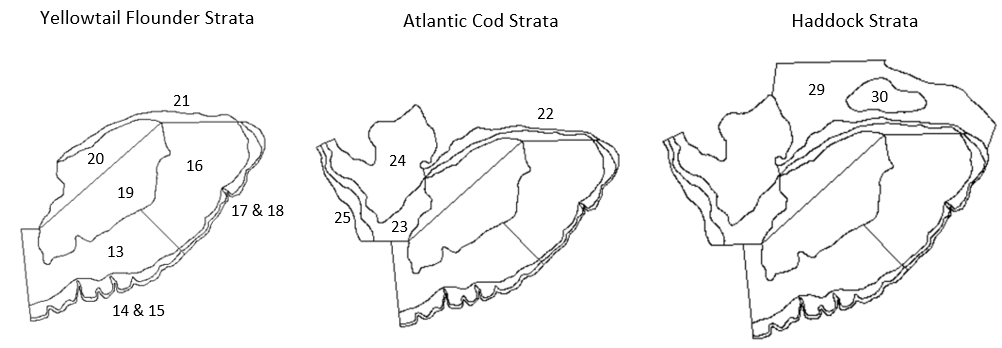
\includegraphics[width=0.95\linewidth]{Images/Strata2} 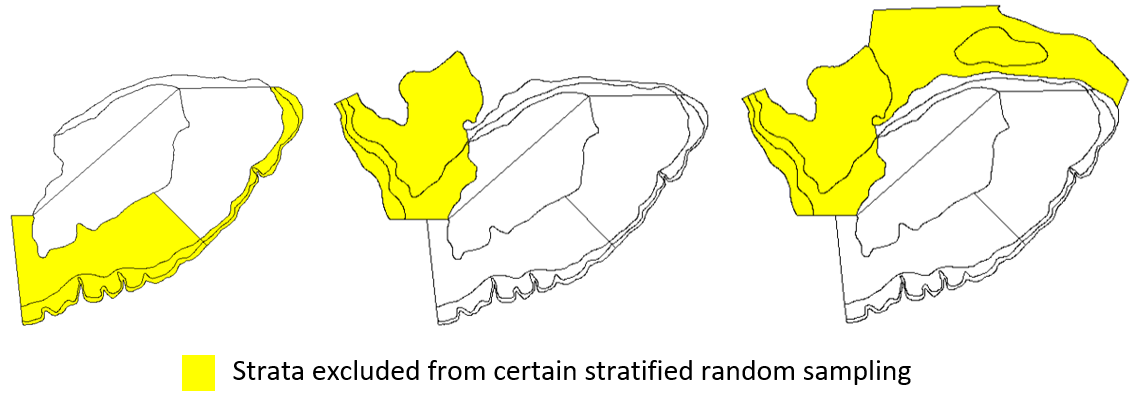
\includegraphics[width=0.95\linewidth]{Images/Excluded_strata2} 

}

\caption{Strata inhabited by each species in our population models.}\label{fig:strata-plot}
\end{figure}

\emph{Population Dynamics and Recruitment}

The time step for our models is one week. MFS uses a modified two-stage Deriso-Schnute delay difference equation that models the biomass in each cell in our study area (Dolder et al. 2020). Individual terms in the formulation account for growth of mature adults, natural and fishing mortality, and the addition of new recruits. We chose to represent recruitment in the model using a Beverton-Holt formulation \textbf{cite}. Recruitment is a function of the adult biomass that existed in the previous year and is added to the population incrementally throughout each species' predefined spawning period. Parameter inputs were either obtained from the literature or chosen to produce desired model dynamics. A full list of parameters used in our model can be seen below in Tables \ref{paramsALL} and \ref{tab:paramsSCENARIOS}.

\emph{Movement}

The package was designed to generate theoretical habitat preferences using Gaussian Random Fields that combine with hypothetical temperature gradients to drive the probability of movement from cell \(I\) to cell \(J\) using the formulation

\begin{align}
Pr(C_{wk+1}=J|C_{wk}=I) = \frac{e^{-\lambda \cdot d_{I,J}}\cdot(Hab^2_{J,s} \cdot Tol_{J,s,wk})}{\sum^C_{c=1}e^{-\lambda \cdot d} \cdot (Hab^2_{c,s} \cdot Tol_{c,s,wk})},
\label{moveP}
\end{align}

where

\(e^{-\lambda \cdot d_{I,J}}\) accounts for distance between cells \(I\) and \(J\),

\(Hab^2_{J,s}\) is the static habitat value for species \(s\) in cell \(J\), and

\(Tol_{c,s,wk}\) is the value from normally distributed temperature tolerance for species \(s\) in cell \(c\) in week \(wk\).

The following sections describe how we formulated the habitat and temperature components to model real species on the northeast continental shelf.

\emph{Habitat Input}

Species-specific habitat preferences were derived using the \emph{lrren} tool from the R package \emph{envi} (Buller 2022) to create a niche model for each species. The \emph{lrren} tool estimates an ecological niche using the relative risk function by relating presence/absence data to two covariate predictors. We used bottom trawl point data in from 2009-2021 as our presence/absence input by using a value of 0 for any tow that failed to catch the given species and weighting a successful catch by the biomass of the given tow {[}{[}I don't think we need to cite the trawl data because we said we were using trawl data above{]}{]} \textbf{BL: Does trawl data ever get cited? It was not cited above. cite trawl data?}. We combined data from both the fall and spring surveys to obscure the influence of temperature so that the niche model would instead infer habitat preferences. Depth and mean sediment size were used as our covariate predictors. Estimated depth for the region was obtained from FVCOM (Chen et al. 2006). The mean sediment size raster was interpolated in ArcMap using the natural neighbor interpolation method \textbf{cite arcmap} using point data collected by the United States Geologic Survey (USGS) (McMullen et al. n.d.). Since the values in \(Hab^2_{J,s}\) are required to be between 0 and 1, we transform the spatial estimates from \emph{lrren} to fall between these bounds. See Figure \ref{fig:hab-plot1} for a visual representation of this process being applied to Cod. Figure \ref{fig:hab-plot} depicts habitat preferences \(Hab^2_{J,s}\) for each species.

\begin{figure}

{\centering 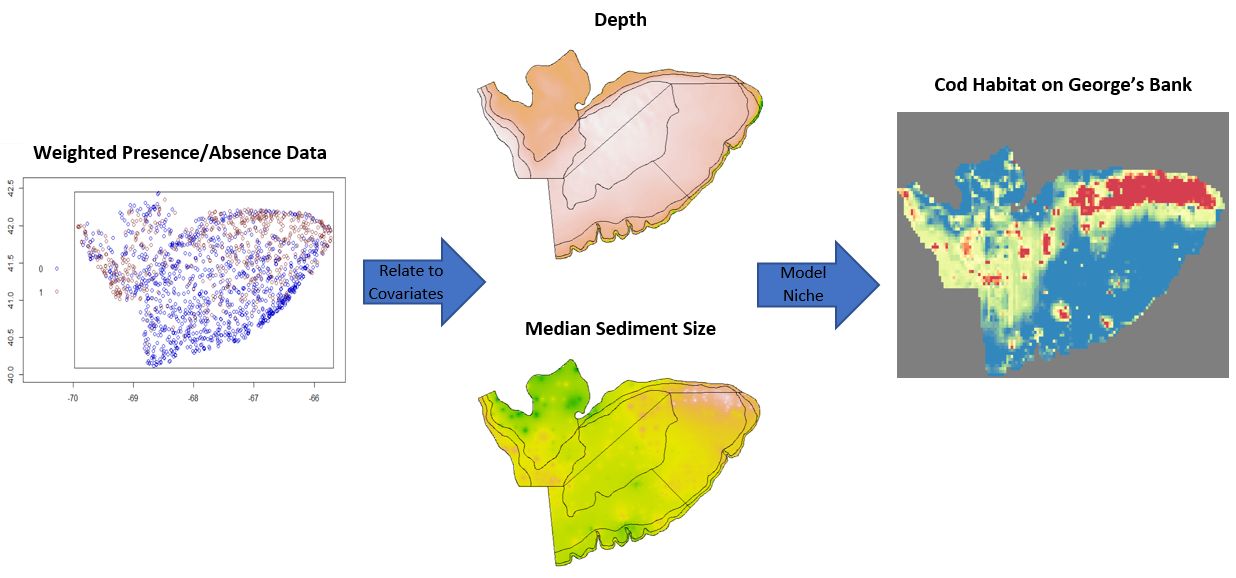
\includegraphics[width=0.95\linewidth]{Images/hab_snip3} 

}

\caption{Visual representation of niche model for Cod.}\label{fig:hab-plot1}
\end{figure}

\begin{figure}

{\centering 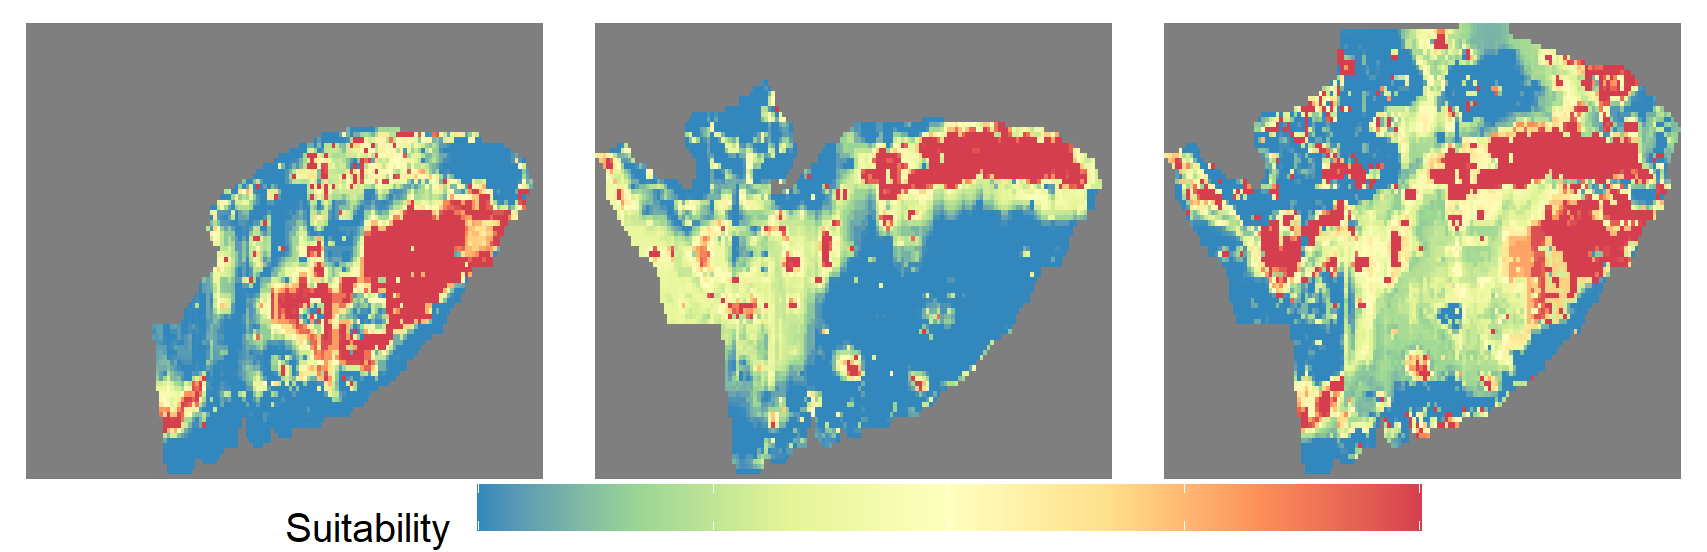
\includegraphics[width=0.95\linewidth]{Images/Habitat_3species} 

}

\caption{Static habitat preferences for each species in our population models (Yellotwtail, Cod, Haddock).}\label{fig:hab-plot}
\end{figure}

\emph{Temperature Input}

Each species is assumed to have normally distributed temperature preferences (\(N(\mu,\sigma)\)). We assume Yellowtail Flounder's preferences are \(N(8.75,4.25)\), while Haddock and Cod have preferences \(N(9,4)\). We chose these values by combining information in the literature with temperatures recorded in the bottom trawl survey. Weekly estimated temperature data for the region for 2012 was obtained from FVCOM (Chen et al. 2006). We chose to repeat estimates for a single year rather than use data for consecutive years to reduce the number of factors impacting model dynamics while still incorporating real data. The 2012 data was chosen because it displayed an average temperature pattern that consistently oscillated between maximum and minimum temperature values, allowing for a smooth repeating yearly temperature pattern for the constant temperature scenario. The 2012 temperature data was also transformed to create an oscillating pattern that increases 5 degrees Celsius on average over the duration of the simulation. We chose a 5 degree increase over a 20 year simulation to allow temperature change to have a meaningful impact on dynamics while remaining within reasonable computational limits in terms of the length of the simulation. Figure \ref{fig:temp-scenarios} depicts mean trends for the temperature scenarios used in our models. \textbf{dont forget to include gif in final submission}

\begin{figure}

{\centering 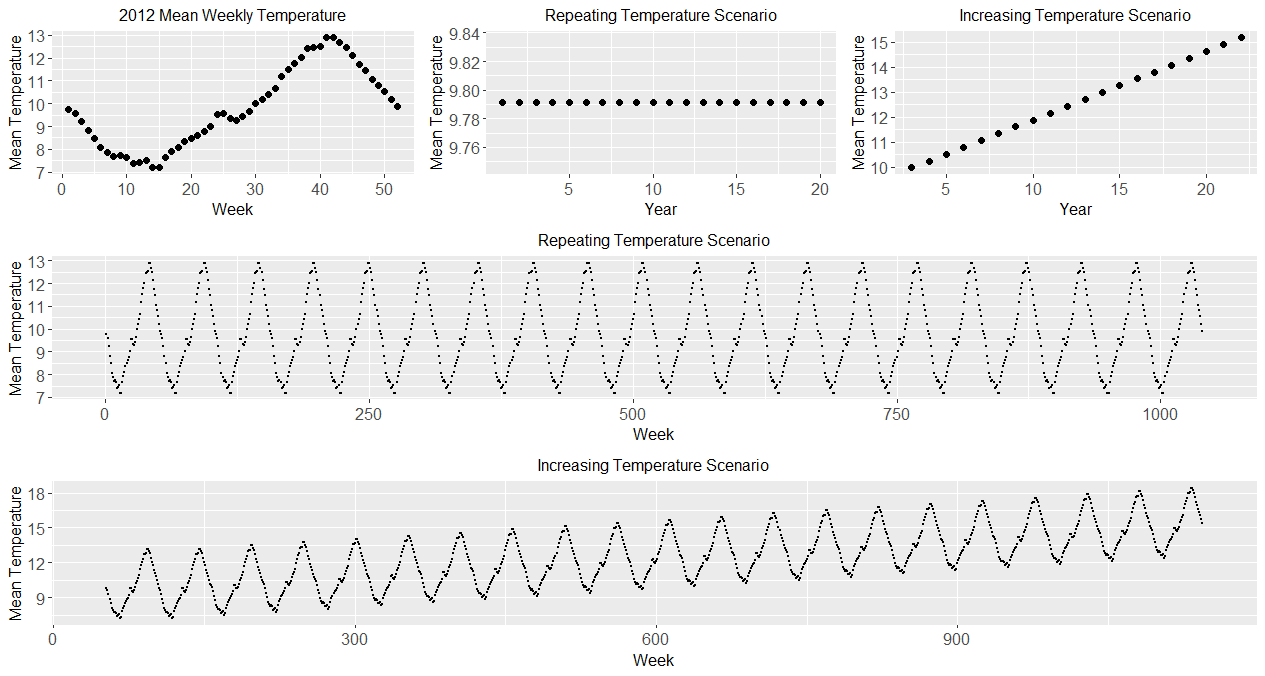
\includegraphics[width=0.95\linewidth]{Images/TempScenarios} 

}

\caption{Mean trends of temperature data used in our model.}\label{fig:temp-scenarios}
\end{figure}

--Describe difference between increasing and constant temperature scenarios (images?)

In equation (1), \(Hab^2_{J,s}\) is constant for the duration of the simulation, while \(Tol_{c,s,wk}\) changes each week. Using a temperature gradient that repeats every 52 weeks produces the same spatial preferences in a given week each year, resulting in consistent spatial biomass patterns. Scenarios where the temperature increases over time creates spatial preferences that evolve as the water warms, producing spatial biomass patterns that shift in a given week over the duration of the simulation. Thus, stratified random samples in scenarios with a repeating temperature pattern will have constant survey catchability and availability over time, which may not be true for increasing temperature scenarios due to evolving spatial preferences.

-- Describe each scenario that is considered

We consider 20 year simulations under three population parameter scenarios for each of our three species- a scenario where parameters result in each population increasing over time, one where the populations are relatively constant over time, and a scenario where the parameter combination results in each population decreasing over time. Each of these three scenarios is paired with a temperature gradient that repeats as well as one that increasing roughly 5 degrees Celsius over the duration of the 20 year simulation. We therefore simulate 6 scenarios for each population.

\emph{Simulating Bottom Trawl Survey and Population Indexing}

-Describe post hoc sampling process and how data is used

After each simulation is complete, we mimic the bottom trawl survey by conducting stratified random sampling in each inhabited strata twice each year. We sample each strata in the same weeks in which the Spring and Fall surveys take place, and the number of the samples taken reflect true target values for each strata. Most strata contain enough cells that we were able to generate a list of sampling locations without replacement, allowing us to sample a unique random cell in each survey over the duration of the simulation. For strata that contain small numbers of cells, we generate a random sampling locations with replacement of cells previously sampled. We then use the biomass collected from our samples in contemporary population indexing methods to estimate population trends. Knowing the true population values in our simulations allows us to compare the error calculated from each estimation method.

--Stratified mean vs VAST with and without covariates

Stock assessment scientists use samples from the bottom trawl survey to estimate the abundance for each fish stock. There are a number of approaches to obtain abundance estimates including traditional design-based estimates to model-based estimates that range in complexity. Design-based estimators rely on the design of the sampling scheme with the underlying assumption that the data being collected is representative of the population of interest. These methods do not account for spatial variation in samples or allow the inclusion of environmental influences. Model-based abundance estimates use statistical models to measure the relationship between response variables (such as presence or abundance) and predictor variables (such as environmental factors). Model-based estimators, such as General Linear Models (GLM), General Additive Model (GAM), and General Linear Mixed Models (GLMM), help account for complex relationships between variables and can help overcome problems with sampling design.

We compare yearly abundance estimates obtained from the stratified mean to estimates obtained from the Vector-Autoregressive Spatio-temporal (VAST) model. The stratified mean is a design-based approach that calculates the geometric mean catch per tow and has traditionally been used with stratified random sample designs. VAST is a spatial delta-generalized linear mixed model that estimates both abundance (biomass) and probability of occurrence (presence/absence) (Thorson 2019). If desired, VAST also allows users to include covariate data to better inform the model. Covariates can be static (eg. habitat preferences) or dynamics (eg. temperature). We explore whether including environmental predictors can help inform models and provide better abundance estimates, which is particularly relevant as climate change progresses. The stratified mean calculations are straightforward and quick, while VAST models require numerous user inputs and can take on the order of hours to complete.

We follow the advice given in (Thorson 2019) to build VAST models to estimate biomass on Georges Bank using stratified random samples from our model output. In addition to exploring different link functions and assumed distributions, our VAST model-building process involved testing the impact of including spatial and/or spatio-temporal variation in our models, considering varying number of knots in our mesh, and testing different forms of temporal correlation. We also carried out the same process running models without covariate information as well as including covariates in our model. We considered covariates in the form of dynamic temperature values and/or static habitat values (\(Hab_{J.s}\)) from our population model. When using covariates we ultimately decided to provide the most information to the model by including both temperature and habitat covariates for both linear predictors. Knowing the true population values in our models allowed us to calculate the absolute error of each VAST estimate to compare between potential settings. Through this process, and in consultation with the VAST package creator, we ultimately compared the performance of two sets of settings in our VAST models, which can be seen in Table\ref{tab:VASTsettings}.

Our goal is to determine indexing approaches and settings that are robust to future environmental conditions and resulting spatial biomass patterns. An underlying assumption in all indexing methods is that individual random samples combine to accurately represent true abundance by a) containing a low enough noise level in the samples to allow for a discernible pattern and b) sampling all strata in which the population exists. These assumptions can be questioned given enough noise in the sampling process \textbf{cite?} and/or climate change causing a population to move into previously uninhabited strata. To simulate the impact of noise, we compare indexing estimates after adding noise to our samples versus those using the true sampling values. \textbf{BL: Help with correct notation for adding noise}. We simulate the effect of populations moving into new habitat by comparing indexing estimates using samples from all strata inhabited by each species on Georges Bank to those that only include a subset of the full spatial domain for each species. We chose strata to exclude for each species by reviewing how spatial preferences evolved in our increasing temperature scenarios and removing strata that each species either shifted into, or away from. Tabl XXX {[}{[}needs to be added{]}{]} lists all strata inhabited by each species, those that are removed from certain calculations, and the explanation of why these strata were removed.

When combining population trends for each species, differing temperature scenarios, altering seasons, and sampling possibilities (noise, strata, covariates) there are a large number of scenario combinations to consider. The columns in Table \ref{tab:scenarios} show the choices that define each scenario.

\begin{table}

\caption{\label{tab:scenarios}Each index estimate chooses one condition from each of the following
7 columns. There are 3*3*2*2*2*2*2 = 288 VAST model combinations and 3*3*2*2*2*2 = 144 stratified mean estimates.}
\centering
\resizebox{\linewidth}{!}{
\begin{tabular}[t]{lllllll}
\toprule
Species & Population Trend & Temperature Scenario & Strata Included & Noise Added & Season & Covariates (VAST)\\
\midrule
Yellowtail & Increasing & Repeating & All strata & No & Spring & No\\
Cod & Constant & Increasing 5°C & Subset & Yes & Fall & Yes\\
Haddock & Decreasing &  &  &  &  & \\
\bottomrule
\end{tabular}}
\end{table}

\section{Results}

The goal of our project was to analyze the ability of contemporary population indexing methods to track population trends under a variety of conditions, as depicted in Table \ref{tab:scenarios}. Historically, Atlantic Cod has seen significant decline over the last XXX years while Haddock has increased in abundance in recent year {[}{[}can cite the 2022 management track assessments, see \url{https://apps-nefsc.fisheries.noaa.gov/saw/sari.php} for when the document becomes available{]}{]} \textbf{cite}. For this reason we compare indexing estimates using stratified random samples from decreasing population scenarios for Cod and increasing population scenarios for Haddock. To provide a comprehensive analysis of population indexing methods we consider all possible scenario combinations for Yellowtail Flounder. The specific population trends used in our analyses can be see in Figure \ref{fig:pop-scenarios}.

\begin{figure}

{\centering 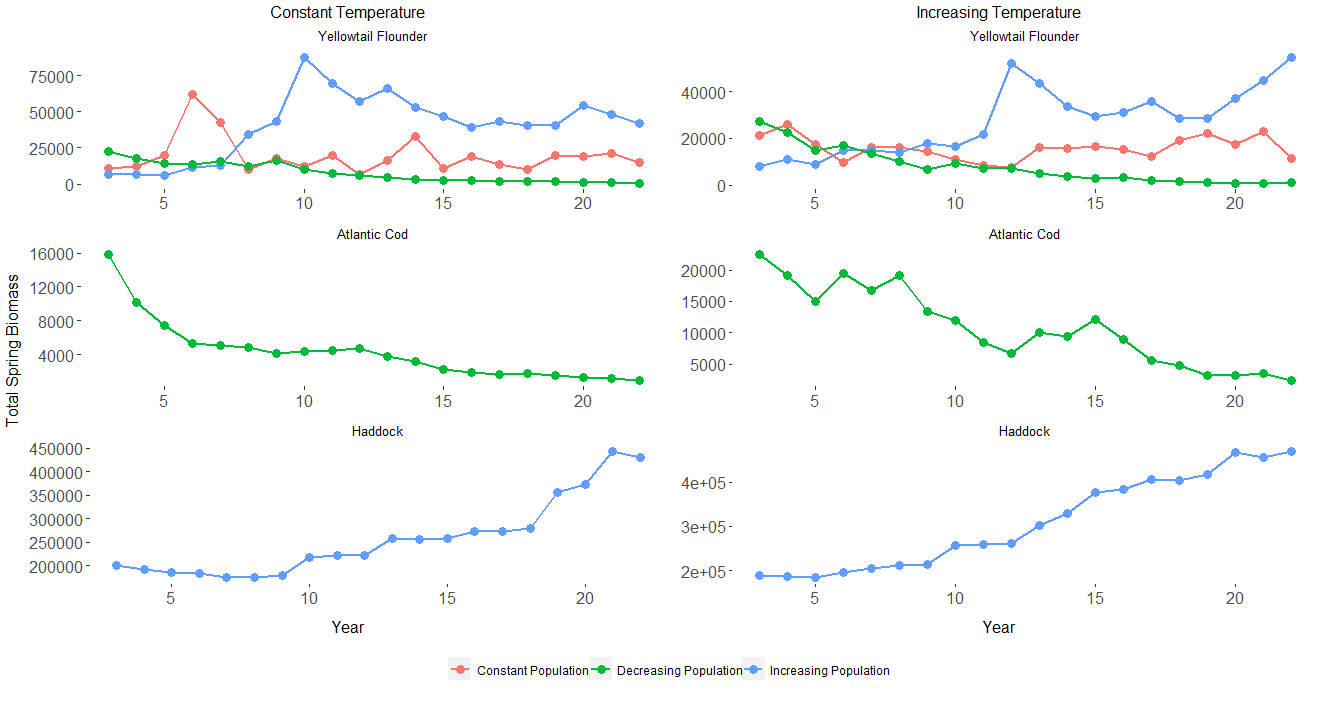
\includegraphics[width=0.99\linewidth]{Images/Population_scenarios} 

}

\caption{True population trends used in indexing analyses. Spring biomass plots are shown with fall values being very similar.}\label{fig:pop-scenarios}
\end{figure}

Tables \ref{tab:YTresultsallstrata}, \ref{tab:YTresultsreducedstrata}, \ref{tab:CodERROR}, and \ref{tab:HadERROR} contain the results of our comparison between the absolute error between abundance estimates and model output. General themes are that VAST estimates provide lower errors relative to those derived from the stratified mean, with VAST models that include covariate information providing the lowest overall errors and standard deviations. On the contrary, we also see individual cases where the stratified mean produced the lowest absolute error. When we reduce the number of strata that are included in indexing calculations to simulate species shifting into new territory, we typically see an increase in absolute error (as expected), though there are some scenarios where the impact is minimal. Furthermore, there are scenarios where including covariates in VAST models actually increases the absolute error, especially when we fail to sample the entire domain.

In considering the Yellowtail Flounder results in Tables \ref{tab:YTresultsallstrata} and \ref{tab:YTresultsreducedstrata}, we can see VAST estimates generally provide lower errors relative to those derived from the stratified mean, with models that include covariate information typically providing the lowest errors. When all strata are included on sampling, adding covariates greatly improved estimates in all scenarios. We still see an improvement in VAST estimates when certain strata are excluded from sampling, but the improvement was much less dramatic than with all strata included. However, there are several instances in which VAST failed to provide improved abundance estimates during the fall season without covariate information, producing the largest errors seen in Tables \ref{tab:YTresultsallstrata} and \ref{tab:YTresultsreducedstrata}. These errors are corrected by including covariate information resulting in improved VAST estimates that are significantly lower than their stratified mean counterparts.

(see Table \ref{tab:CodERROR}) In the Cod results, when using reduced strata in constant temperature, adding covariates produces worse VAST results (though still better than stratified mean). This is similar to what we see with all of Haddock results (adding covariates makes it worse with reduced strata). This is NOT seen with Yellowtail (adding covariates always helps). VAST without covariates much worse than stratified mean in fall with increasing temperature, but adding covariates corrects this and makes VAST estimates better than stratified mean.

(see Table \ref{tab:HadERROR}) For Haddock, VAST has a particularly hard time in spring regularly producing larger errors than the stratified mean with added covariates only improving to the level of the stratified mean. VAST shows improved results in fall relative to the stratified mean with added covariates producing extremely low errors in some cases. In Haddock results, adding covariates improves estimates only when all strata are included (when reduced strata, adding covariates actually makes VAST worse). Since this occurs in all scenarios, it seems to again be related to failing to accurately monitor strata 17.

\emph{Differences Between VAST Settings}

For YTF, 29/96 \textasciitilde{} 30\% of VAST runs with new settings were better (70\% were worse). 80/96 \textasciitilde{} 83\% of scenarios had a VAST run with a better error than the stratified mean. 15/16 of the times the stratified mean was better VAST was not using covariates. The 1 time that VAST was using covariates and was still worse than the stratified mean was IncPop\_IncTemp\_Allstrata\_WCov\_WNoise in the Fall (VAST had strong overestimate in the fall during IncPOP\_IncTemP\_allstrata for Had and YT). The overestimate in the fall only seems to be related to the way the population shifts between season. Looking at the percent shift plots, the population is shifting out of strata 16 in both seasons (large east strata). In the spring the population is shifting mostly into strata 17 (thin strata adjacent to 16), but in the fall they are shifting into both 17 and 18 (18 thin one adjacent to 17). Thus it seems like with much of the population concentrated in the really small outer most strata, VAST produces an underestimate, even with covariates

For Haddock (IncPop), 18/32 \textasciitilde{} 57\% of VAST runs better with new settings. 24/32 = 75\% of scenarios had a VAST run with a better error than the stratified mean. 14/16 VAST were better with covariates (the two that were worse were essentially the same) while only 10/16 were better without covariates. Stratified mean tended to perform better when all strata were included in the calculation, while VAST tended to perform better when strata are removed.

For Cod (DecPop), only 11/32 \textasciitilde{} 34\% of VAST runs were better with new settings. 28/32\textasciitilde{} 88\% of scenarios had a VAST run with a better estimate than the stratified mean. All 16/16 = 100\% of VAST runs with a covariate were better than the stratified mean. 12/16 VAST were better without covariates. The 4 runs without covariates that were worse were all extremely large errors and all from increasing temp in the fall (with and without all strata and noise). In the fall the population is moving out of strata 16 (large eastern strata) and 21 (north large) and into a number of strata (22 (tiny north), 24 (large north), 18 (tiny north)). Might be having trouble tracking in to smaller strata again.

{[}{[}We'll want to expand the results section to focus on the impact of each factor one at at time within each species. This will be a bit dull, but it is important to walk through the results in words to ensure that readers get the message. They can of course examine the tables in detail and draw their own conclusions, but we should put our interpretation down on paper.{]}{]}

Figure \ref{fig:PopPct} depicts the spatial shifting that occurs in each strata within our population models, specifically during the bottom trawl survey weeks in the spring (13 and 14) and fall (37 and 28). See Figure \ref{fig:strata-plot} for a spatial reference of the Georges Bank strata and Figure \ref{fig:hab-plot} for the static habitat preferences for each species (\(Hab^2_{J,s}\)) used in our population models.

\emph{Yellowtail Flounder Results}

The top two panels in Figure \ref{fig:PopPct} depict the results for Yellowtail Flounder with a repeating temperature gradient on the left (constant temperature) and a temperature gradient that increases over time on the right (increasing temperature). In both temperature scenarios we see the percent of Yellowtail Flounder in strata 13 decrease over the course of the time series in both seasons. The spring population in stratum 19 also decreases in both temperature scenarios as well. The percent of the population increases in stratum 16 in the spring over the duration of both time series, which implies the flow out of strata 13 and 19 in the spring are going into stratum 16. These dynamics occur in both temperature scenarios in weeks 13 and 14 because stratum 16 contains favorable habitat for Yellowtail Flounder that coincides with most of the areas we have designated as the species' spawning ground, which takes place in weeks 9-12. These spring dynamics are therefore related to the static habitat values in our model rather than the dynamics temperature preferences. While we observe similar dynamics in the fall (weeks 37 and 38) in the constant temperature scenario, an increasing average temperature results in a decrease in population in stratum 16 over time and corresponding increases in strata 17 and 18 (see Figure \ref{fig:PopPct}). These dynamics imply that an increase in temperature results in the more shallow strata 16 becoming less desirable than the deeper and more narrow exterior strata 17 and 18. One noticeable seasonal difference in the constant temperature scenario for Yellowtail is how \textasciitilde10\% of the population exists in the narrow exterior strata 17 in the fall, while seemingly none of the population exists in any of the exterior strata (14, 15, 17, 18) in the spring.

Tables \ref{tab:YTresultsallstrata} and \ref{tab:YTresultsreducedstrata} contain the absolute error between our abundance estimates for Yellowtail Flounder comparing design-based approach (stratified mean) with two settings for a model-based approach (VAST A \& B). Of all scenarios without covariates, \(33/48\approx68\)\% had a VAST fit with a lower relative error compared to the stratified mean estimate. All 15 of the covariate-free VAST estimates that resulted in a higher error than the stratified mean were for the fall season and had a common theme of producing abundance estimates that are above the true model value. These 15 fall estimates span all other scenario variations. The implication of this is that our model-based approach without covariates struggles with the primary seasonal difference for Yellowtail Flounder, which is that a larger percentage of the population exists in the narrow exterior strata (18 and/or 17). This theory is further supported by the fact that the absolute error in the increasing temperature scenarios increased dramatically in the fall season, when the combined percentage of the population in the outer strata 17 and 18 increased to over 40\% by the end of the simulation.

Including detailed covariate information made a noticeable difference in our Yellowtail Flounder model-based VAST estimates. All of the VAST estimates that included covariate information produced a lower relative error than the corresponding VAST model that did not include covariates. The largest improvements were seen in the increasing temperature scenarios. As a result, of the VAST estimates that included covariates information, \(47/48\approx98\)\% had a lower relative error than the corresponding stratified mean estimate. This implies that the covariate information helped our model-based estimate account for the design-based issues related to small strata that contain a large percentage of the population, which can become exacerbated in the increasing temperature scenario.

The performance of our abundance estimates tend to decrease under increasing temperature, with the most dramatic changes seen in our VAST estimates without covariates. One exception to this is when we use a stratified mean approach while the population is decreasing. Our analyses have found that the stratified mean tends to under estimate the true abundance and since these estimates are bounded below by zero, as the Yellowtail population decreases towards zero the difference between the estimate and the true value also decrease. That is, if the population is low enough, failing to appropriately sample the population in a design-based method produces the same result as appropriately sampling.

\textbf{For discussion: clearly our perfect covariate information made a big difference here, but the question is could we achieve similar results without ``perfect'' information? Which covariate is best? Good question for future research}

\emph{Cod Results}

We see a seasonal impact of an increasing average temperature in stratum 16 in the Cod results in Figure \ref{fig:PopPct}. In the constant temperature scenario for Cod, in both seasons the population is decreasing its presence in strata 19 and 20 over the duration of the simulation, while simultaneously increasing presence in stratum 16. However, an increase in average temperature in the fall drives the population out of strata 16 and 21, and into 18, 22, and 24 (see Figure \ref{fig:hab-plot}). Similar to the Yellowtail Flounder population, stratum the habitat in stratum 16 acts as an attractor in both temperature scenarios in the spring when the water temperature is cooler. When the temperature increases over time the fall population begins to prefer the adjacent strata that are deeper and/or more northern than stratum 16.

Of the abundance estimates without covariates, \(12/16=75\)\% had a VAST fit with a lower relative error compared to the stratified mean estimate. Including detailed covariate information in our Cod VAST estimates resulted in all \(16/16=100\%\) having a lower relative error than the corresponding stratified mean estimate. The 4 scenarios without covariates that had a higher VAST error were each overestimates for the fall season that involved an increasing temperature gradient. Similar to Yellowtail Flounder results, Cod are shifting their spatial distribution into the smaller exterior strata in these conditions, which is decreasing the accuracy of the covariate-free VAST estimate. While adding covariates to these fits allowed for an improved error relative to the stratified mean, the VAST abundance still display an overestimate early in the time series before covariates correct the trend, allowing for a lower overall absolute error \textbf{(show these plots? IncTemp fall scenarios)}.

\emph{Haddock Results}

Figure \ref{fig:PopPct} reveals some subtle seasonal differences in the percent of haddock in each strata. In the constant temperature scenarios, the spring shows a decrease in strata 19 and 20 that correspond to increases in 16, 24 and 29. This change represents a northward movement between larger centrally located strata. While strata 24 and 29 also increase in the fall under constant temperature, the corresponding decrease is primarily from strata 16 and 13. While similar results can be seen in the spring for the increasing temperature scenario, much more dramatic results exist in the fall under increasing temperature as we see a significant decreases in strata 13, 16, 21, and 22 that leads to the most noticeable increases in strata 17, 18, and 29. This shift represents movement from the shallower and more centrally located strata towards exterior deeper strata. Since stratum 16 contains very favorable habitat including much of the species' spawning ground, the strong shift out of 16 and into the northern most strata of 29 in the fall demonstrates a climate-driven change in movement preference.

\(10/16\approx63\)\% of the scenarios without covariates had a VAST fit with a lower relative error compared to the stratified mean estimate. The 6 covariate-free VAST estimates that resulted in a higher error than the stratified mean spanned all scenarios and seasons, with several fall errors being especially large (significant overestimates). Adding covariate information resulted in \(14/16\approx88\)\% of VAST estimates having improved error compared to the stratified mean. The 2 scenarios that procedure worse error spanned temperature scenarios, but were both in the spring season when the proportion of the population in each strata remained constant in each scenario.\textbf{why?? doesnt make sense. the values with cov are about the same as SM} Qualitatively, including covariate information has a larger impact on decreasing the relative error compared to the stratified mean compared to failing to include covariates.

\emph{Model / Estimate Ratio Results}

A simple visual analysis of all error plots for each species reveals that VAST estimates tend to provide abundance estimates that are above the true model value, while the stratified mean estimates are, on average, too low. This can be further examined by viewing estimate/ratio ratio plots, where we divide the yearly abundance estimates by the true model value. In doing so we see that VAST estimates tend to remain closer to the desired value of 1 compared to stratified mean estimates, which can range as low as 0 and exhibit large yearly changes.

A more careful analysis of individual yearly model/estimate ratios when all strata are included revealed that about 73\% of all VAST ratios were above 1 (27\% less than 1), with an average of 1.29 and a standard deviation of 0.21. On the other hand, 33\% of stratified mean estimates were above 1 with an average of 0.874 and a standard deviation of 0.12. There were seasonal differences in estimate ratios with spring VAST ratios producing (1.08,0.12), fall VAST ratios being (1.50,0.38), stratified mean spring ratios resulting in (0.91,0.10), and fall values of (0.84,0.16). The breakdown for individual species followed a similar pattern.

When the entire domain is sampled, adding covariates brings the estimate ratio closer to 1. However, when failing to sample the entire domain, adding covariates can decrease the accuracy of VAST estimates. When including all strata, the stratified mean produced (0.87,0.12), while adding covariates improved the VAST estimate ratio from (1.45,0.17) to (1.13,0.09). With a reduced number of strata, the stratified mean resulted in our worst summary values of (0.59,0.10), and adding covariates to our VAST models decreased the average ratio results from (1.04,0.33 ) to (0.78,0.19).

\section{Discussion}

Estimation methods that have large, inaccurate swings (stratified mean) can lead to changes in quotas that do not correspond to the true population trend, which could have a compounding effect (can lead to quotas that are too high/low given an incorrect assumption of increase/decrease in biomass). Our model has a constant assumed mortality that accounts for fishing and natural death and will not account for impacts of these decisions. VAST may provide more consistent biomass predictions(?)

{[}{[} some things that I think we'll need to address, in addition to those mentioned above are (in no particular order):
number of simulations done for each scenario - time required to do them and analyses
pros and cons of using VAST with covariates in a changing environment
implications for current practice of using stratified mean (not horrible, but might be able to do better with model-based using covariates if enviro changing, note we don't want to say stratified mean should not be used because that will draw a lot of tomato throwing)
future work - some of the ideas we've discussed already could be mentioned
limitations to our study
perhaps for discussion, but we should mention somewhere that MFS only tracks biomass not age structure, the latter is important for stock assessments but not considered in this paper{]}{]}

\section{Acknowledgements}

{[}{[}we should thank Jim (obviously), but also those who helped you with the habitat data (robyn, david Chev.) and others? also should note that funding provided by Climate-Groundfish source (I'll dig up the official name of the funding source){]}{]}

\hypertarget{data-and-code-availability}{%
\subsection{Data and Code Availability}\label{data-and-code-availability}}

All data and code used in this work are available at \url{https://github.com/Blevy2/READ-PDB-blevy2-MFS2}.

\hypertarget{references}{%
\subsection{References}\label{references}}

\hypertarget{refs}{}
\begin{CSLReferences}{1}{0}
\leavevmode\vadjust pre{\hypertarget{ref-azarovitz1981brief}{}}%
Azarovitz, T. 1981. A brief historical review of the woods hole laboratory trawl survey time series. Bottom trawl surveys.

\leavevmode\vadjust pre{\hypertarget{ref-envi}{}}%
Buller, I.D. 2022. Envi: Environmental interpolation using spatial kernel density estimation. The Comprehensive R Archive Network. doi:\href{https://doi.org/10.5281/zenodo.5347826}{10.5281/zenodo.5347826}.

\leavevmode\vadjust pre{\hypertarget{ref-chen2006unstructured}{}}%
Chen, C., Beardsley, R.C., Cowles, G., Qi, J., Lai, Z., Gao, G., and others. 2006. An unstructured grid, finite-volume coastal ocean model: FVCOM user manual. SMAST/UMASSD: 6--8.

\leavevmode\vadjust pre{\hypertarget{ref-dolder2020highly}{}}%
Dolder, P.J., Minto, C., Guarini, J.-M., and Poos, J.J. 2020. Highly resolved spatiotemporal simulations for exploring mixed fishery dynamics. Ecological Modelling \textbf{424}: 109000. Elsevier.

\leavevmode\vadjust pre{\hypertarget{ref-mcmullen2005usgs}{}}%
McMullen, K., Paskevich, V., and Poppe, L. (n.d.). USGS east-coast sediment analysis: Procedures, database, and GIS data. US Geological Survey Open-File Report \textbf{2005}: 1001.

\leavevmode\vadjust pre{\hypertarget{ref-politis2014northeast}{}}%
Politis, P.J., Galbraith, J.K., Kostovick, P., and Brown, R.W. 2014. Northeast fisheries science center bottom trawl survey protocols for the NOAA ship henry b. bigelow.

\leavevmode\vadjust pre{\hypertarget{ref-thorson2019guidance}{}}%
Thorson, J.T. 2019. Guidance for decisions using the vector autoregressive spatio-temporal (VAST) package in stock, ecosystem, habitat and climate assessments. Fisheries Research \textbf{210}: 143--161. Elsevier.

\end{CSLReferences}

\pagebreak

\hypertarget{tables}{%
\subsection{Tables}\label{tables}}

\pagebreak

\begin{figure}

{\centering 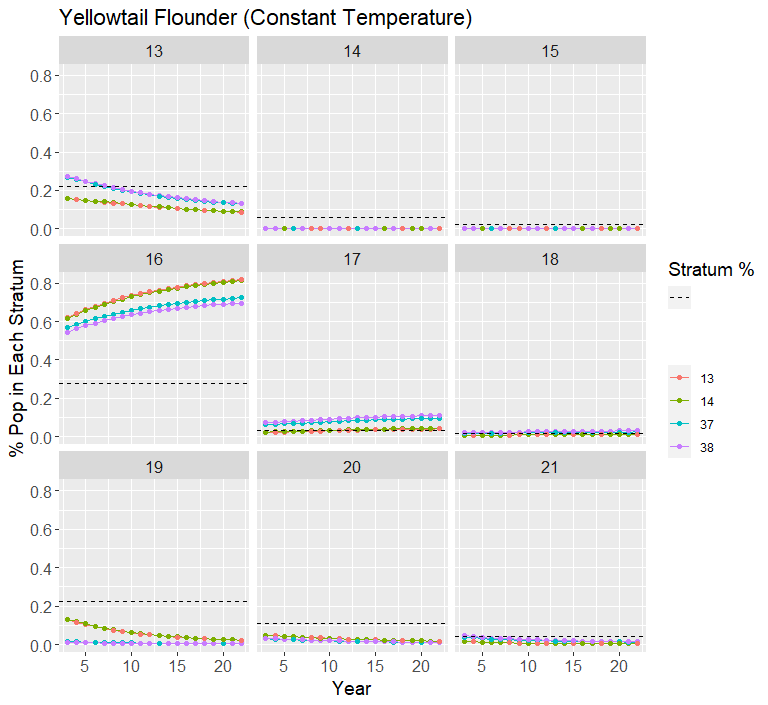
\includegraphics[width=0.475\linewidth]{Images/PercentPlots_ConPopConTemp_YT} 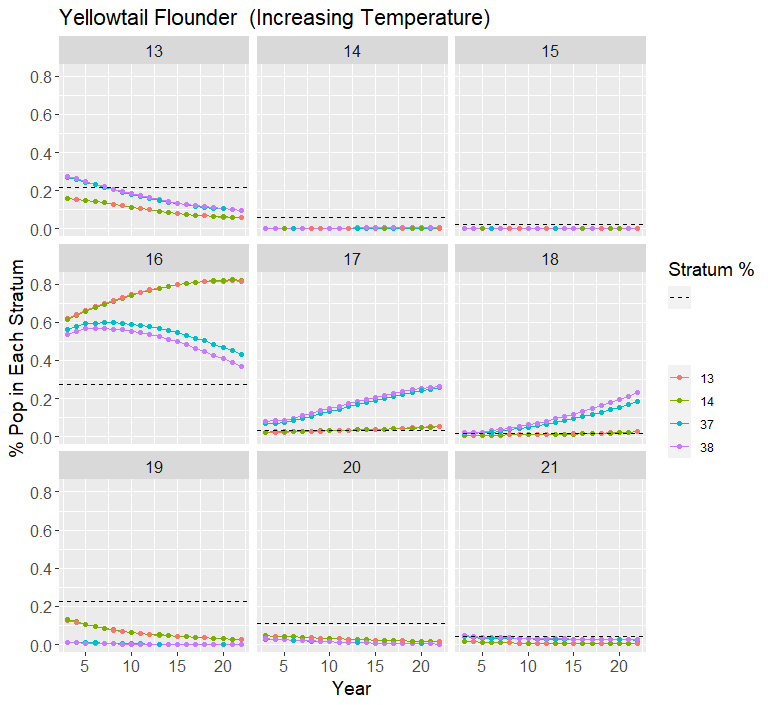
\includegraphics[width=0.475\linewidth]{Images/PercentPlots_ConPopIncTemp_YT} 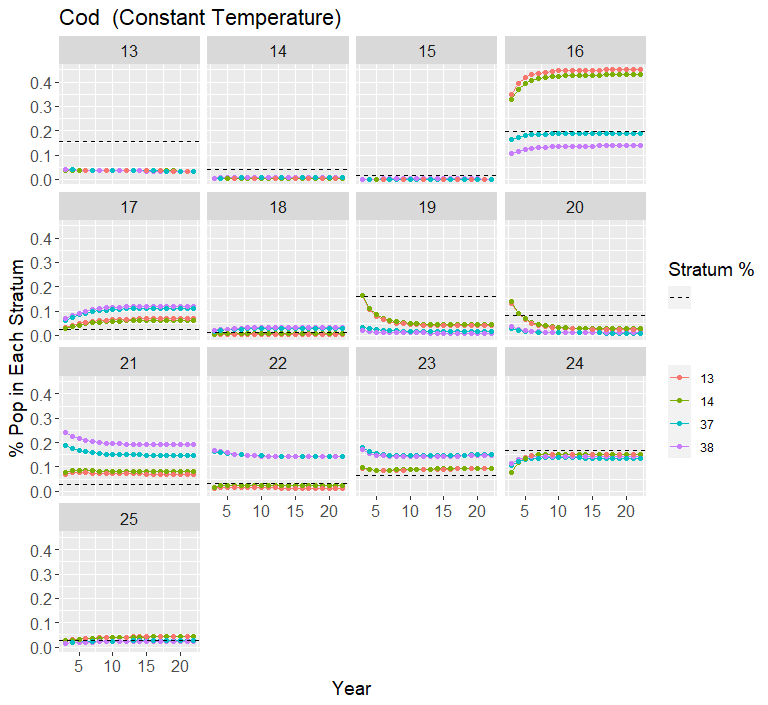
\includegraphics[width=0.475\linewidth]{Images/PercentPlots_DecPopConTemp_Cod} 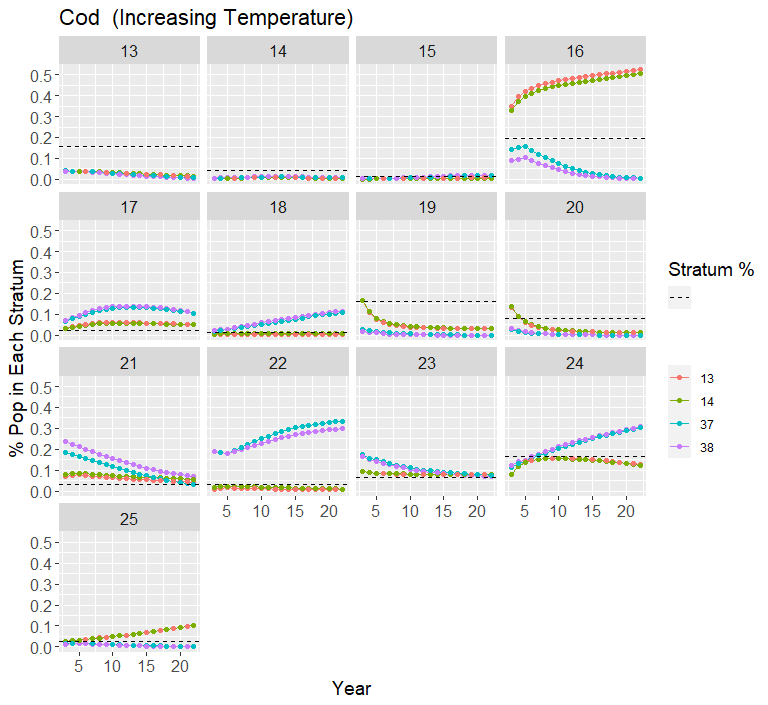
\includegraphics[width=0.475\linewidth]{Images/PercentPlots_DecPopIncTemp_Cod} 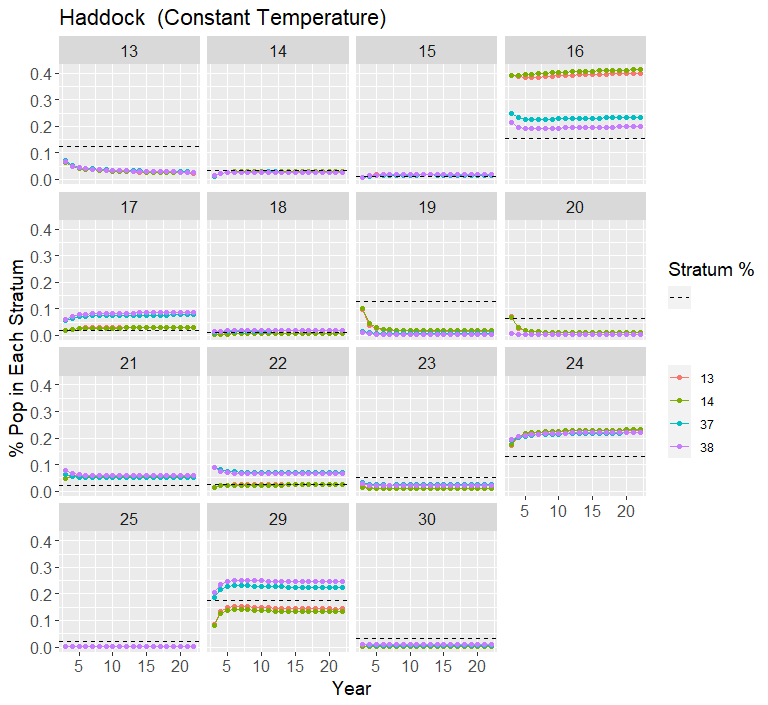
\includegraphics[width=0.475\linewidth]{Images/PercentPlots_IncPopConTemp_Had} 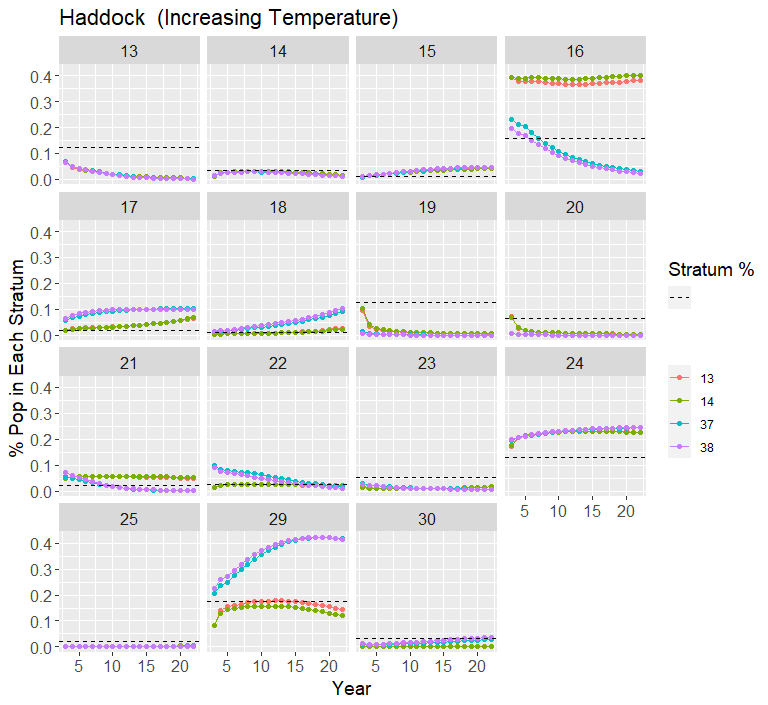
\includegraphics[width=0.475\linewidth]{Images/PercentPlots_IncPopIncTemp_Had} 

}

\caption{Percent of each species in each strata for during survey weeks in our spatial simulations. All constant temperature scenarios follow the patterns on the left while increasing temperature scenarios follow the patterns on the right.}\label{fig:PopPct}
\end{figure}

Table 1. Parameters used in all population models.

\begin{longtable}[]{@{}lllllll@{}}
\toprule
Parameter & Description & Unit & Yellowtail & Cod & Haddock & Source \\
\midrule
\endhead
\(\rho\) & Ford's growth coefficient & wk\(^{-1}\) & 4.48 & 4.43 & 4.49 & \\
\(M\) & Natural Mortality & wk\(^{-1}\) & 0.2064 & 0.2728 & 0.3340 & \\
\(W_R\) & Weight of fully recruited fish & kg & 0.39 & 2.95 & 1.12 & \\
\(W_{R-1}\) & Weight of pre-recruit fish & kg & 0.13 & 0.39 & 0.19 & \\
\(\sigma^2\) & Variance in recruited fish & kg\(^2\) & 0.55 & 0.55 & 0.55 & \\
\(\lambda\) & Decay rate for movement & - & 0.7 & 0.7 & 0.7 & \\
\(Spwn_s\) & Spawning weeks for species \(s\) & wk & 9-12 & 8-13 & 11-14 & \\
\(Rec_s\) & Recruitment weeks for species \(s\) & wk & 9-12 & 8-13 & 11-14 & \\
\bottomrule
\end{longtable}

\begin{table}
 
 \caption{\label{tab:paramsALL2}Parameters used in all population models.}
 \centering
 \fontsize{10}{12}\selectfont
 \begin{tabular}[t]{lllllll}
 \toprule
 Parameter & Description & Unit & Yellowtail & Cod & Haddock & Source\\
 \midrule
 <U+03C1> & Ford's growth coefficient & 1/wk & 4.48 & 4.43 & 4.49 & \\
 M & Natural mortality & 1/wk & 0.2064 & 0.2728 & 0.334 & \\
 W1 & Weight of fully recruited fish & kg & 0.39 & 2.95 & 1.12 & \\
 W2 & Weight of pre-recruit fish & kg & 0.13 & 0.39 & 0.19 & \\
 sigma & Variance in recruited fish & kg*kg & 0.55 & 0.55 & 0.55 & \\
 \addlinespace
 lambda & Decay rate for movement & - & 0.7 & 0.7 & 0.7 & \\
 spwn & Spawning weeks for species s & wks & 9-12 & 8-13 & 11-14 & \\
 rec & Recruitment weeks for species s & wks & 9-12 & 8-13 & 11-14 & \\
 \bottomrule
 \end{tabular}
 \end{table}

\begin{table}

\caption{\label{tab:paramsSCENARIOS}Parameters used in population models for each scenario.}
\centering
\fontsize{10}{12}\selectfont
\begin{tabular}[t]{llllll}
\toprule
Parameter & Description & Unit & Yellowtail & Cod & Haddock\\
\midrule
\addlinespace[0.3em]
\multicolumn{1}{l}{\textbf{Constant Population}}\\
\hspace{1em}M+F & Adjusted Mortality (Natural + Fishing) & 1/wk & 0.764 & 0.83 & 0.309\\
\hspace{1em}P0 & Initial Biomass & kg & 3190 & 21500 & \vphantom{1} 180000\\
\hspace{1em}a & Max recruitment rate & kg & 30400 & 27900 & 73600\\
\hspace{1em}ß & Recruitment half saturation value & kg & 4300 & 10500 & 40500\\
\addlinespace[0.3em]
\multicolumn{1}{l}{\textbf{Decreasing Population}}\\
\hspace{1em}M+F & Adjusted Mortality (Natural + Fishing) & 1/wk & 0.764 & 0.623 & 0.334\\
\hspace{1em}P0 & Initial Biomass & kg & 50000 & 21500 & 180000\\
\hspace{1em}a & Max recruitment rate & kg & 1.07e+12 & 3.89e+08 & 4.97e+08\\
\hspace{1em}ß & Recruitment half saturation value & kg & 2.3e+12 & 9.8e+08 & 2.08e+09\\
\addlinespace[0.3em]
\multicolumn{1}{l}{\textbf{Increasing Population}}\\
\hspace{1em}M+F & Adjusted Mortality (Natural + Fishing) & 1/wk & 0.564 & 0.372 & 0.134\\
\hspace{1em}P0 & Initial Biomass & kg & 3190 & 21500 & 180000\\
\hspace{1em}a & Max recruitment rate & kg & 40000 & 45000 & 1e+05\\
\hspace{1em}ß & Recruitment half saturation value & kg & 43000 & 62800 & 405000\\
\bottomrule
\end{tabular}
\end{table}

Table XX. Parameters used in all VAST models.

\begin{longtable}[]{@{}
  >{\raggedright\arraybackslash}p{(\columnwidth - 6\tabcolsep) * \real{0.14}}
  >{\raggedright\arraybackslash}p{(\columnwidth - 6\tabcolsep) * \real{0.38}}
  >{\raggedright\arraybackslash}p{(\columnwidth - 6\tabcolsep) * \real{0.24}}
  >{\raggedright\arraybackslash}p{(\columnwidth - 6\tabcolsep) * \real{0.24}}@{}}
\toprule
\begin{minipage}[b]{\linewidth}\raggedright
Parameter
\end{minipage} & \begin{minipage}[b]{\linewidth}\raggedright
Description
\end{minipage} & \begin{minipage}[b]{\linewidth}\raggedright
Settings A
\end{minipage} & \begin{minipage}[b]{\linewidth}\raggedright
Settings B
\end{minipage} \\
\midrule
\endhead
\emph{ObsModel} & Link function and assumed distribution & c(10,2) & c(10,2) \\
FieldConfig & Specified spatial and/or spatio-temporal variation in predictors & c(Omega1=0, Epsilon1=0, Omega2=1, Epsilon2=1) & c(Omega1=0, Epsilon1=0, Omega2=1, Epsilon2=1) \\
RhoConfig & Specifying whether intercepts or spatio-temporal variation is structured among time intervals & c(Beta1=3, Beta2=, Epsilon1=0, Epsilon2=4) & c(Beta1=3, Beta2=3, Epsilon1=0, Epsilon2=4) \\
X1\_formula & Right-sided formula affecting the 1st linear predictor & X1\_formula = \textasciitilde{} poly(Temp, degree=2 ) & N/A \\
X2\_formula & Right-sided formula affecting the 2nd linear predictor & X2\_formula = \textasciitilde{} poly(Temp, degree=2 ) + poly(Habitat, degree=2 ) & X2\_formula = \textasciitilde{} poly(Temp, degree=2 ) + poly(Habitat, degree=2 ) \\
\bottomrule
\end{longtable}

\begin{table}

\caption{\label{tab:YTresultsallstrata}Yellowtail flounder error results with all strata included in calculations. Row colors correspond to the same settings applied in different seasons.}
\centering
\fontsize{10}{12}\selectfont
\begin{tabular}[t]{l|l|l|l|c|c|c}
\hline
\textbf{Temperature Scenario} & \textbf{Season} & \textbf{Covariate} & \textbf{Noise} & \textbf{VAST A} & \textbf{VAST B} & \textbf{Stratified Mean}\\
\hline
\multicolumn{1}{l}{\textbf{Constant Population}}\\
\hline
\cellcolor{black}{\textcolor{white}{\textbf{\hspace{1em}Constant}}} & \cellcolor{black}{\textcolor{white}{\textbf{spring}}} & \cellcolor{black}{\textcolor{white}{\textbf{no cov}}} & \cellcolor{black}{\textcolor{white}{\textbf{no}}} & \cellcolor{black}{\textcolor{white}{\textbf{0.13}}} & \cellcolor{black}{\textcolor{white}{\textbf{0.11}}} & \cellcolor{black}{\textcolor{white}{\textbf{0.21}}}\\
\hline
\cellcolor[HTML]{5C5E60}{\textcolor{white}{\textbf{\hspace{1em}Constant}}} & \cellcolor[HTML]{5C5E60}{\textcolor{white}{\textbf{spring}}} & \cellcolor[HTML]{5C5E60}{\textcolor{white}{\textbf{no cov}}} & \cellcolor[HTML]{5C5E60}{\textcolor{white}{\textbf{yes}}} & \cellcolor[HTML]{5C5E60}{\textcolor{white}{\textbf{0.14}}} & \cellcolor[HTML]{5C5E60}{\textcolor{white}{\textbf{0.16}}} & \cellcolor[HTML]{5C5E60}{\textcolor{white}{\textbf{0.25}}}\\
\hline
\cellcolor[HTML]{A4A4A4}{\textcolor{white}{\textbf{\hspace{1em}Constant}}} & \cellcolor[HTML]{A4A4A4}{\textcolor{white}{\textbf{spring}}} & \cellcolor[HTML]{A4A4A4}{\textcolor{white}{\textbf{w/ cov}}} & \cellcolor[HTML]{A4A4A4}{\textcolor{white}{\textbf{no}}} & \cellcolor[HTML]{A4A4A4}{\textcolor{white}{\textbf{0.07}}} & \cellcolor[HTML]{A4A4A4}{\textcolor{white}{\textbf{0.07}}} & \cellcolor[HTML]{A4A4A4}{\textcolor{white}{\textbf{0.21}}}\\
\hline
\cellcolor[HTML]{D2D2D2}{\textcolor{white}{\textbf{\hspace{1em}Constant}}} & \cellcolor[HTML]{D2D2D2}{\textcolor{white}{\textbf{spring}}} & \cellcolor[HTML]{D2D2D2}{\textcolor{white}{\textbf{w/ cov}}} & \cellcolor[HTML]{D2D2D2}{\textcolor{white}{\textbf{yes}}} & \cellcolor[HTML]{D2D2D2}{\textcolor{white}{\textbf{0.08}}} & \cellcolor[HTML]{D2D2D2}{\textcolor{white}{\textbf{0.08}}} & \cellcolor[HTML]{D2D2D2}{\textcolor{white}{\textbf{0.25}}}\\
\hline
\cellcolor{black}{\textcolor{white}{\textbf{\hspace{1em}Constant}}} & \cellcolor{black}{\textcolor{white}{\textbf{fall}}} & \cellcolor{black}{\textcolor{white}{\textbf{no cov}}} & \cellcolor{black}{\textcolor{white}{\textbf{no}}} & \cellcolor{black}{\textcolor{white}{\textbf{0.63}}} & \cellcolor{black}{\textcolor{white}{\textbf{0.68}}} & \cellcolor{black}{\textcolor{white}{\textbf{0.32}}}\\
\hline
\cellcolor[HTML]{5C5E60}{\textcolor{white}{\textbf{\hspace{1em}Constant}}} & \cellcolor[HTML]{5C5E60}{\textcolor{white}{\textbf{fall}}} & \cellcolor[HTML]{5C5E60}{\textcolor{white}{\textbf{no cov}}} & \cellcolor[HTML]{5C5E60}{\textcolor{white}{\textbf{yes}}} & \cellcolor[HTML]{5C5E60}{\textcolor{white}{\textbf{0.80}}} & \cellcolor[HTML]{5C5E60}{\textcolor{white}{\textbf{0.77}}} & \cellcolor[HTML]{5C5E60}{\textcolor{white}{\textbf{0.31}}}\\
\hline
\cellcolor[HTML]{A4A4A4}{\textcolor{white}{\textbf{\hspace{1em}Constant}}} & \cellcolor[HTML]{A4A4A4}{\textcolor{white}{\textbf{fall}}} & \cellcolor[HTML]{A4A4A4}{\textcolor{white}{\textbf{w/ cov}}} & \cellcolor[HTML]{A4A4A4}{\textcolor{white}{\textbf{no}}} & \cellcolor[HTML]{A4A4A4}{\textcolor{white}{\textbf{0.14}}} & \cellcolor[HTML]{A4A4A4}{\textcolor{white}{\textbf{0.08}}} & \cellcolor[HTML]{A4A4A4}{\textcolor{white}{\textbf{0.32}}}\\
\hline
\cellcolor[HTML]{D2D2D2}{\textcolor{white}{\textbf{\hspace{1em}Constant}}} & \cellcolor[HTML]{D2D2D2}{\textcolor{white}{\textbf{fall}}} & \cellcolor[HTML]{D2D2D2}{\textcolor{white}{\textbf{w/ cov}}} & \cellcolor[HTML]{D2D2D2}{\textcolor{white}{\textbf{yes}}} & \cellcolor[HTML]{D2D2D2}{\textcolor{white}{\textbf{0.17}}} & \cellcolor[HTML]{D2D2D2}{\textcolor{white}{\textbf{0.11}}} & \cellcolor[HTML]{D2D2D2}{\textcolor{white}{\textbf{0.31}}}\\
\hline
\cellcolor{black}{\textcolor{white}{\textbf{\hspace{1em}Increasing}}} & \cellcolor{black}{\textcolor{white}{\textbf{spring}}} & \cellcolor{black}{\textcolor{white}{\textbf{no cov}}} & \cellcolor{black}{\textcolor{white}{\textbf{no}}} & \cellcolor{black}{\textcolor{white}{\textbf{0.14}}} & \cellcolor{black}{\textcolor{white}{\textbf{0.11}}} & \cellcolor{black}{\textcolor{white}{\textbf{0.28}}}\\
\hline
\cellcolor[HTML]{5C5E60}{\textcolor{white}{\textbf{\hspace{1em}Increasing}}} & \cellcolor[HTML]{5C5E60}{\textcolor{white}{\textbf{spring}}} & \cellcolor[HTML]{5C5E60}{\textcolor{white}{\textbf{no cov}}} & \cellcolor[HTML]{5C5E60}{\textcolor{white}{\textbf{yes}}} & \cellcolor[HTML]{5C5E60}{\textcolor{white}{\textbf{0.18}}} & \cellcolor[HTML]{5C5E60}{\textcolor{white}{\textbf{0.15}}} & \cellcolor[HTML]{5C5E60}{\textcolor{white}{\textbf{0.28}}}\\
\hline
\cellcolor[HTML]{A4A4A4}{\textcolor{white}{\textbf{\hspace{1em}Increasing}}} & \cellcolor[HTML]{A4A4A4}{\textcolor{white}{\textbf{spring}}} & \cellcolor[HTML]{A4A4A4}{\textcolor{white}{\textbf{w/ cov}}} & \cellcolor[HTML]{A4A4A4}{\textcolor{white}{\textbf{no}}} & \cellcolor[HTML]{A4A4A4}{\textcolor{white}{\textbf{0.05}}} & \cellcolor[HTML]{A4A4A4}{\textcolor{white}{\textbf{0.06}}} & \cellcolor[HTML]{A4A4A4}{\textcolor{white}{\textbf{0.28}}}\\
\hline
\cellcolor[HTML]{D2D2D2}{\textcolor{white}{\textbf{\hspace{1em}Increasing}}} & \cellcolor[HTML]{D2D2D2}{\textcolor{white}{\textbf{spring}}} & \cellcolor[HTML]{D2D2D2}{\textcolor{white}{\textbf{w/ cov}}} & \cellcolor[HTML]{D2D2D2}{\textcolor{white}{\textbf{yes}}} & \cellcolor[HTML]{D2D2D2}{\textcolor{white}{\textbf{0.10}}} & \cellcolor[HTML]{D2D2D2}{\textcolor{white}{\textbf{0.12}}} & \cellcolor[HTML]{D2D2D2}{\textcolor{white}{\textbf{0.28}}}\\
\hline
\cellcolor{black}{\textcolor{white}{\textbf{\hspace{1em}Increasing}}} & \cellcolor{black}{\textcolor{white}{\textbf{fall}}} & \cellcolor{black}{\textcolor{white}{\textbf{no cov}}} & \cellcolor{black}{\textcolor{white}{\textbf{no}}} & \cellcolor{black}{\textcolor{white}{\textbf{1.46}}} & \cellcolor{black}{\textcolor{white}{\textbf{1.26}}} & \cellcolor{black}{\textcolor{white}{\textbf{0.51}}}\\
\hline
\cellcolor[HTML]{5C5E60}{\textcolor{white}{\textbf{\hspace{1em}Increasing}}} & \cellcolor[HTML]{5C5E60}{\textcolor{white}{\textbf{fall}}} & \cellcolor[HTML]{5C5E60}{\textcolor{white}{\textbf{no cov}}} & \cellcolor[HTML]{5C5E60}{\textcolor{white}{\textbf{yes}}} & \cellcolor[HTML]{5C5E60}{\textcolor{white}{\textbf{1.40}}} & \cellcolor[HTML]{5C5E60}{\textcolor{white}{\textbf{1.38}}} & \cellcolor[HTML]{5C5E60}{\textcolor{white}{\textbf{0.50}}}\\
\hline
\cellcolor[HTML]{A4A4A4}{\textcolor{white}{\textbf{\hspace{1em}Increasing}}} & \cellcolor[HTML]{A4A4A4}{\textcolor{white}{\textbf{fall}}} & \cellcolor[HTML]{A4A4A4}{\textcolor{white}{\textbf{w/ cov}}} & \cellcolor[HTML]{A4A4A4}{\textcolor{white}{\textbf{no}}} & \cellcolor[HTML]{A4A4A4}{\textcolor{white}{\textbf{0.21}}} & \cellcolor[HTML]{A4A4A4}{\textcolor{white}{\textbf{0.23}}} & \cellcolor[HTML]{A4A4A4}{\textcolor{white}{\textbf{0.51}}}\\
\hline
\cellcolor[HTML]{D2D2D2}{\textcolor{white}{\textbf{\hspace{1em}Increasing}}} & \cellcolor[HTML]{D2D2D2}{\textcolor{white}{\textbf{fall}}} & \cellcolor[HTML]{D2D2D2}{\textcolor{white}{\textbf{w/ cov}}} & \cellcolor[HTML]{D2D2D2}{\textcolor{white}{\textbf{yes}}} & \cellcolor[HTML]{D2D2D2}{\textcolor{white}{\textbf{0.30}}} & \cellcolor[HTML]{D2D2D2}{\textcolor{white}{\textbf{0.28}}} & \cellcolor[HTML]{D2D2D2}{\textcolor{white}{\textbf{0.50}}}\\
\hline
\multicolumn{1}{l}{\textbf{Decreasing Population}}\\
\hline
\cellcolor{black}{\textcolor{white}{\textbf{\hspace{1em}Constant}}} & \cellcolor{black}{\textcolor{white}{\textbf{spring}}} & \cellcolor{black}{\textcolor{white}{\textbf{no cov}}} & \cellcolor{black}{\textcolor{white}{\textbf{no}}} & \cellcolor{black}{\textcolor{white}{\textbf{0.11}}} & \cellcolor{black}{\textcolor{white}{\textbf{0.08}}} & \cellcolor{black}{\textcolor{white}{\textbf{0.23}}}\\
\hline
\cellcolor[HTML]{5C5E60}{\textcolor{white}{\textbf{\hspace{1em}Constant}}} & \cellcolor[HTML]{5C5E60}{\textcolor{white}{\textbf{spring}}} & \cellcolor[HTML]{5C5E60}{\textcolor{white}{\textbf{no cov}}} & \cellcolor[HTML]{5C5E60}{\textcolor{white}{\textbf{yes}}} & \cellcolor[HTML]{5C5E60}{\textcolor{white}{\textbf{0.12}}} & \cellcolor[HTML]{5C5E60}{\textcolor{white}{\textbf{0.11}}} & \cellcolor[HTML]{5C5E60}{\textcolor{white}{\textbf{0.27}}}\\
\hline
\cellcolor[HTML]{A4A4A4}{\textcolor{white}{\textbf{\hspace{1em}Constant}}} & \cellcolor[HTML]{A4A4A4}{\textcolor{white}{\textbf{spring}}} & \cellcolor[HTML]{A4A4A4}{\textcolor{white}{\textbf{w/ cov}}} & \cellcolor[HTML]{A4A4A4}{\textcolor{white}{\textbf{no}}} & \cellcolor[HTML]{A4A4A4}{\textcolor{white}{\textbf{0.07}}} & \cellcolor[HTML]{A4A4A4}{\textcolor{white}{\textbf{0.06}}} & \cellcolor[HTML]{A4A4A4}{\textcolor{white}{\textbf{0.23}}}\\
\hline
\cellcolor[HTML]{D2D2D2}{\textcolor{white}{\textbf{\hspace{1em}Constant}}} & \cellcolor[HTML]{D2D2D2}{\textcolor{white}{\textbf{spring}}} & \cellcolor[HTML]{D2D2D2}{\textcolor{white}{\textbf{w/ cov}}} & \cellcolor[HTML]{D2D2D2}{\textcolor{white}{\textbf{yes}}} & \cellcolor[HTML]{D2D2D2}{\textcolor{white}{\textbf{0.11}}} & \cellcolor[HTML]{D2D2D2}{\textcolor{white}{\textbf{0.07}}} & \cellcolor[HTML]{D2D2D2}{\textcolor{white}{\textbf{0.27}}}\\
\hline
\cellcolor{black}{\textcolor{white}{\textbf{\hspace{1em}Constant}}} & \cellcolor{black}{\textcolor{white}{\textbf{fall}}} & \cellcolor{black}{\textcolor{white}{\textbf{no cov}}} & \cellcolor{black}{\textcolor{white}{\textbf{no}}} & \cellcolor{black}{\textcolor{white}{\textbf{0.97}}} & \cellcolor{black}{\textcolor{white}{\textbf{0.81}}} & \cellcolor{black}{\textcolor{white}{\textbf{0.41}}}\\
\hline
\cellcolor[HTML]{5C5E60}{\textcolor{white}{\textbf{\hspace{1em}Constant}}} & \cellcolor[HTML]{5C5E60}{\textcolor{white}{\textbf{fall}}} & \cellcolor[HTML]{5C5E60}{\textcolor{white}{\textbf{no cov}}} & \cellcolor[HTML]{5C5E60}{\textcolor{white}{\textbf{yes}}} & \cellcolor[HTML]{5C5E60}{\textcolor{white}{\textbf{0.99}}} & \cellcolor[HTML]{5C5E60}{\textcolor{white}{\textbf{1.09}}} & \cellcolor[HTML]{5C5E60}{\textcolor{white}{\textbf{0.37}}}\\
\hline
\cellcolor[HTML]{A4A4A4}{\textcolor{white}{\textbf{\hspace{1em}Constant}}} & \cellcolor[HTML]{A4A4A4}{\textcolor{white}{\textbf{fall}}} & \cellcolor[HTML]{A4A4A4}{\textcolor{white}{\textbf{w/ cov}}} & \cellcolor[HTML]{A4A4A4}{\textcolor{white}{\textbf{no}}} & \cellcolor[HTML]{A4A4A4}{\textcolor{white}{\textbf{0.16}}} & \cellcolor[HTML]{A4A4A4}{\textcolor{white}{\textbf{0.08}}} & \cellcolor[HTML]{A4A4A4}{\textcolor{white}{\textbf{0.41}}}\\
\hline
\cellcolor[HTML]{D2D2D2}{\textcolor{white}{\textbf{\hspace{1em}Constant}}} & \cellcolor[HTML]{D2D2D2}{\textcolor{white}{\textbf{fall}}} & \cellcolor[HTML]{D2D2D2}{\textcolor{white}{\textbf{w/ cov}}} & \cellcolor[HTML]{D2D2D2}{\textcolor{white}{\textbf{yes}}} & \cellcolor[HTML]{D2D2D2}{\textcolor{white}{\textbf{0.29}}} & \cellcolor[HTML]{D2D2D2}{\textcolor{white}{\textbf{0.18}}} & \cellcolor[HTML]{D2D2D2}{\textcolor{white}{\textbf{0.37}}}\\
\hline
\cellcolor{black}{\textcolor{white}{\textbf{\hspace{1em}Increasing}}} & \cellcolor{black}{\textcolor{white}{\textbf{spring}}} & \cellcolor{black}{\textcolor{white}{\textbf{no cov}}} & \cellcolor{black}{\textcolor{white}{\textbf{no}}} & \cellcolor{black}{\textcolor{white}{\textbf{0.17}}} & \cellcolor{black}{\textcolor{white}{\textbf{0.15}}} & \cellcolor{black}{\textcolor{white}{\textbf{0.22}}}\\
\hline
\cellcolor[HTML]{5C5E60}{\textcolor{white}{\textbf{\hspace{1em}Increasing}}} & \cellcolor[HTML]{5C5E60}{\textcolor{white}{\textbf{spring}}} & \cellcolor[HTML]{5C5E60}{\textcolor{white}{\textbf{no cov}}} & \cellcolor[HTML]{5C5E60}{\textcolor{white}{\textbf{yes}}} & \cellcolor[HTML]{5C5E60}{\textcolor{white}{\textbf{0.15}}} & \cellcolor[HTML]{5C5E60}{\textcolor{white}{\textbf{0.17}}} & \cellcolor[HTML]{5C5E60}{\textcolor{white}{\textbf{0.26}}}\\
\hline
\cellcolor[HTML]{A4A4A4}{\textcolor{white}{\textbf{\hspace{1em}Increasing}}} & \cellcolor[HTML]{A4A4A4}{\textcolor{white}{\textbf{spring}}} & \cellcolor[HTML]{A4A4A4}{\textcolor{white}{\textbf{w/ cov}}} & \cellcolor[HTML]{A4A4A4}{\textcolor{white}{\textbf{no}}} & \cellcolor[HTML]{A4A4A4}{\textcolor{white}{\textbf{0.08}}} & \cellcolor[HTML]{A4A4A4}{\textcolor{white}{\textbf{0.07}}} & \cellcolor[HTML]{A4A4A4}{\textcolor{white}{\textbf{0.22}}}\\
\hline
\cellcolor[HTML]{D2D2D2}{\textcolor{white}{\textbf{\hspace{1em}Increasing}}} & \cellcolor[HTML]{D2D2D2}{\textcolor{white}{\textbf{spring}}} & \cellcolor[HTML]{D2D2D2}{\textcolor{white}{\textbf{w/ cov}}} & \cellcolor[HTML]{D2D2D2}{\textcolor{white}{\textbf{yes}}} & \cellcolor[HTML]{D2D2D2}{\textcolor{white}{\textbf{0.16}}} & \cellcolor[HTML]{D2D2D2}{\textcolor{white}{\textbf{0.10}}} & \cellcolor[HTML]{D2D2D2}{\textcolor{white}{\textbf{0.26}}}\\
\hline
\cellcolor{black}{\textcolor{white}{\textbf{\hspace{1em}Increasing}}} & \cellcolor{black}{\textcolor{white}{\textbf{fall}}} & \cellcolor{black}{\textcolor{white}{\textbf{no cov}}} & \cellcolor{black}{\textcolor{white}{\textbf{no}}} & \cellcolor{black}{\textcolor{white}{\textbf{1.17}}} & \cellcolor{black}{\textcolor{white}{\textbf{1.06}}} & \cellcolor{black}{\textcolor{white}{\textbf{0.28}}}\\
\hline
\cellcolor[HTML]{5C5E60}{\textcolor{white}{\textbf{\hspace{1em}Increasing}}} & \cellcolor[HTML]{5C5E60}{\textcolor{white}{\textbf{fall}}} & \cellcolor[HTML]{5C5E60}{\textcolor{white}{\textbf{no cov}}} & \cellcolor[HTML]{5C5E60}{\textcolor{white}{\textbf{yes}}} & \cellcolor[HTML]{5C5E60}{\textcolor{white}{\textbf{1.14}}} & \cellcolor[HTML]{5C5E60}{\textcolor{white}{\textbf{1.10}}} & \cellcolor[HTML]{5C5E60}{\textcolor{white}{\textbf{0.25}}}\\
\hline
\cellcolor[HTML]{A4A4A4}{\textcolor{white}{\textbf{\hspace{1em}Increasing}}} & \cellcolor[HTML]{A4A4A4}{\textcolor{white}{\textbf{fall}}} & \cellcolor[HTML]{A4A4A4}{\textcolor{white}{\textbf{w/ cov}}} & \cellcolor[HTML]{A4A4A4}{\textcolor{white}{\textbf{no}}} & \cellcolor[HTML]{A4A4A4}{\textcolor{white}{\textbf{0.40}}} & \cellcolor[HTML]{A4A4A4}{\textcolor{white}{\textbf{0.15}}} & \cellcolor[HTML]{A4A4A4}{\textcolor{white}{\textbf{0.28}}}\\
\hline
\cellcolor[HTML]{D2D2D2}{\textcolor{white}{\textbf{\hspace{1em}Increasing}}} & \cellcolor[HTML]{D2D2D2}{\textcolor{white}{\textbf{fall}}} & \cellcolor[HTML]{D2D2D2}{\textcolor{white}{\textbf{w/ cov}}} & \cellcolor[HTML]{D2D2D2}{\textcolor{white}{\textbf{yes}}} & \cellcolor[HTML]{D2D2D2}{\textcolor{white}{\textbf{0.40}}} & \cellcolor[HTML]{D2D2D2}{\textcolor{white}{\textbf{0.20}}} & \cellcolor[HTML]{D2D2D2}{\textcolor{white}{\textbf{0.25}}}\\
\hline
\multicolumn{1}{l}{\textbf{Increasing Population}}\\
\hline
\cellcolor{black}{\textcolor{white}{\textbf{\hspace{1em}Constant}}} & \cellcolor{black}{\textcolor{white}{\textbf{spring}}} & \cellcolor{black}{\textcolor{white}{\textbf{no cov}}} & \cellcolor{black}{\textcolor{white}{\textbf{no}}} & \cellcolor{black}{\textcolor{white}{\textbf{0.46}}} & \cellcolor{black}{\textcolor{white}{\textbf{0.13}}} & \cellcolor{black}{\textcolor{white}{\textbf{0.16}}}\\
\hline
\cellcolor[HTML]{5C5E60}{\textcolor{white}{\textbf{\hspace{1em}Constant}}} & \cellcolor[HTML]{5C5E60}{\textcolor{white}{\textbf{spring}}} & \cellcolor[HTML]{5C5E60}{\textcolor{white}{\textbf{no cov}}} & \cellcolor[HTML]{5C5E60}{\textcolor{white}{\textbf{yes}}} & \cellcolor[HTML]{5C5E60}{\textcolor{white}{\textbf{0.43}}} & \cellcolor[HTML]{5C5E60}{\textcolor{white}{\textbf{0.21}}} & \cellcolor[HTML]{5C5E60}{\textcolor{white}{\textbf{0.22}}}\\
\hline
\cellcolor[HTML]{A4A4A4}{\textcolor{white}{\textbf{\hspace{1em}Constant}}} & \cellcolor[HTML]{A4A4A4}{\textcolor{white}{\textbf{spring}}} & \cellcolor[HTML]{A4A4A4}{\textcolor{white}{\textbf{w/ cov}}} & \cellcolor[HTML]{A4A4A4}{\textcolor{white}{\textbf{no}}} & \cellcolor[HTML]{A4A4A4}{\textcolor{white}{\textbf{0.06}}} & \cellcolor[HTML]{A4A4A4}{\textcolor{white}{\textbf{0.06}}} & \cellcolor[HTML]{A4A4A4}{\textcolor{white}{\textbf{0.16}}}\\
\hline
\cellcolor[HTML]{D2D2D2}{\textcolor{white}{\textbf{\hspace{1em}Constant}}} & \cellcolor[HTML]{D2D2D2}{\textcolor{white}{\textbf{spring}}} & \cellcolor[HTML]{D2D2D2}{\textcolor{white}{\textbf{w/ cov}}} & \cellcolor[HTML]{D2D2D2}{\textcolor{white}{\textbf{yes}}} & \cellcolor[HTML]{D2D2D2}{\textcolor{white}{\textbf{0.08}}} & \cellcolor[HTML]{D2D2D2}{\textcolor{white}{\textbf{0.07}}} & \cellcolor[HTML]{D2D2D2}{\textcolor{white}{\textbf{0.22}}}\\
\hline
\cellcolor{black}{\textcolor{white}{\textbf{\hspace{1em}Constant}}} & \cellcolor{black}{\textcolor{white}{\textbf{fall}}} & \cellcolor{black}{\textcolor{white}{\textbf{no cov}}} & \cellcolor{black}{\textcolor{white}{\textbf{no}}} & \cellcolor{black}{\textcolor{white}{\textbf{0.40}}} & \cellcolor{black}{\textcolor{white}{\textbf{0.36}}} & \cellcolor{black}{\textcolor{white}{\textbf{0.34}}}\\
\hline
\cellcolor[HTML]{5C5E60}{\textcolor{white}{\textbf{\hspace{1em}Constant}}} & \cellcolor[HTML]{5C5E60}{\textcolor{white}{\textbf{fall}}} & \cellcolor[HTML]{5C5E60}{\textcolor{white}{\textbf{no cov}}} & \cellcolor[HTML]{5C5E60}{\textcolor{white}{\textbf{yes}}} & \cellcolor[HTML]{5C5E60}{\textcolor{white}{\textbf{0.38}}} & \cellcolor[HTML]{5C5E60}{\textcolor{white}{\textbf{0.44}}} & \cellcolor[HTML]{5C5E60}{\textcolor{white}{\textbf{0.46}}}\\
\hline
\cellcolor[HTML]{A4A4A4}{\textcolor{white}{\textbf{\hspace{1em}Constant}}} & \cellcolor[HTML]{A4A4A4}{\textcolor{white}{\textbf{fall}}} & \cellcolor[HTML]{A4A4A4}{\textcolor{white}{\textbf{w/ cov}}} & \cellcolor[HTML]{A4A4A4}{\textcolor{white}{\textbf{no}}} & \cellcolor[HTML]{A4A4A4}{\textcolor{white}{\textbf{0.11}}} & \cellcolor[HTML]{A4A4A4}{\textcolor{white}{\textbf{0.08}}} & \cellcolor[HTML]{A4A4A4}{\textcolor{white}{\textbf{0.34}}}\\
\hline
\cellcolor[HTML]{D2D2D2}{\textcolor{white}{\textbf{\hspace{1em}Constant}}} & \cellcolor[HTML]{D2D2D2}{\textcolor{white}{\textbf{fall}}} & \cellcolor[HTML]{D2D2D2}{\textcolor{white}{\textbf{w/ cov}}} & \cellcolor[HTML]{D2D2D2}{\textcolor{white}{\textbf{yes}}} & \cellcolor[HTML]{D2D2D2}{\textcolor{white}{\textbf{0.24}}} & \cellcolor[HTML]{D2D2D2}{\textcolor{white}{\textbf{0.17}}} & \cellcolor[HTML]{D2D2D2}{\textcolor{white}{\textbf{0.46}}}\\
\hline
\cellcolor{black}{\textcolor{white}{\textbf{\hspace{1em}Increasing}}} & \cellcolor{black}{\textcolor{white}{\textbf{spring}}} & \cellcolor{black}{\textcolor{white}{\textbf{no cov}}} & \cellcolor{black}{\textcolor{white}{\textbf{no}}} & \cellcolor{black}{\textcolor{white}{\textbf{0.16}}} & \cellcolor{black}{\textcolor{white}{\textbf{0.13}}} & \cellcolor{black}{\textcolor{white}{\textbf{0.32}}}\\
\hline
\cellcolor[HTML]{5C5E60}{\textcolor{white}{\textbf{\hspace{1em}Increasing}}} & \cellcolor[HTML]{5C5E60}{\textcolor{white}{\textbf{spring}}} & \cellcolor[HTML]{5C5E60}{\textcolor{white}{\textbf{no cov}}} & \cellcolor[HTML]{5C5E60}{\textcolor{white}{\textbf{yes}}} & \cellcolor[HTML]{5C5E60}{\textcolor{white}{\textbf{0.21}}} & \cellcolor[HTML]{5C5E60}{\textcolor{white}{\textbf{0.16}}} & \cellcolor[HTML]{5C5E60}{\textcolor{white}{\textbf{0.32}}}\\
\hline
\cellcolor[HTML]{A4A4A4}{\textcolor{white}{\textbf{\hspace{1em}Increasing}}} & \cellcolor[HTML]{A4A4A4}{\textcolor{white}{\textbf{spring}}} & \cellcolor[HTML]{A4A4A4}{\textcolor{white}{\textbf{w/ cov}}} & \cellcolor[HTML]{A4A4A4}{\textcolor{white}{\textbf{no}}} & \cellcolor[HTML]{A4A4A4}{\textcolor{white}{\textbf{0.06}}} & \cellcolor[HTML]{A4A4A4}{\textcolor{white}{\textbf{0.07}}} & \cellcolor[HTML]{A4A4A4}{\textcolor{white}{\textbf{0.32}}}\\
\hline
\cellcolor[HTML]{D2D2D2}{\textcolor{white}{\textbf{\hspace{1em}Increasing}}} & \cellcolor[HTML]{D2D2D2}{\textcolor{white}{\textbf{spring}}} & \cellcolor[HTML]{D2D2D2}{\textcolor{white}{\textbf{w/ cov}}} & \cellcolor[HTML]{D2D2D2}{\textcolor{white}{\textbf{yes}}} & \cellcolor[HTML]{D2D2D2}{\textcolor{white}{\textbf{0.12}}} & \cellcolor[HTML]{D2D2D2}{\textcolor{white}{\textbf{0.10}}} & \cellcolor[HTML]{D2D2D2}{\textcolor{white}{\textbf{0.32}}}\\
\hline
\cellcolor{black}{\textcolor{white}{\textbf{\hspace{1em}Increasing}}} & \cellcolor{black}{\textcolor{white}{\textbf{fall}}} & \cellcolor{black}{\textcolor{white}{\textbf{no cov}}} & \cellcolor{black}{\textcolor{white}{\textbf{no}}} & \cellcolor{black}{\textcolor{white}{\textbf{0.71}}} & \cellcolor{black}{\textcolor{white}{\textbf{0.66}}} & \cellcolor{black}{\textcolor{white}{\textbf{0.30}}}\\
\hline
\cellcolor[HTML]{5C5E60}{\textcolor{white}{\textbf{\hspace{1em}Increasing}}} & \cellcolor[HTML]{5C5E60}{\textcolor{white}{\textbf{fall}}} & \cellcolor[HTML]{5C5E60}{\textcolor{white}{\textbf{no cov}}} & \cellcolor[HTML]{5C5E60}{\textcolor{white}{\textbf{yes}}} & \cellcolor[HTML]{5C5E60}{\textcolor{white}{\textbf{1.03}}} & \cellcolor[HTML]{5C5E60}{\textcolor{white}{\textbf{0.71}}} & \cellcolor[HTML]{5C5E60}{\textcolor{white}{\textbf{0.39}}}\\
\hline
\cellcolor[HTML]{A4A4A4}{\textcolor{white}{\textbf{\hspace{1em}Increasing}}} & \cellcolor[HTML]{A4A4A4}{\textcolor{white}{\textbf{fall}}} & \cellcolor[HTML]{A4A4A4}{\textcolor{white}{\textbf{w/ cov}}} & \cellcolor[HTML]{A4A4A4}{\textcolor{white}{\textbf{no}}} & \cellcolor[HTML]{A4A4A4}{\textcolor{white}{\textbf{0.43}}} & \cellcolor[HTML]{A4A4A4}{\textcolor{white}{\textbf{0.21}}} & \cellcolor[HTML]{A4A4A4}{\textcolor{white}{\textbf{0.30}}}\\
\hline
\cellcolor[HTML]{D2D2D2}{\textcolor{white}{\textbf{\hspace{1em}Increasing}}} & \cellcolor[HTML]{D2D2D2}{\textcolor{white}{\textbf{fall}}} & \cellcolor[HTML]{D2D2D2}{\textcolor{white}{\textbf{w/ cov}}} & \cellcolor[HTML]{D2D2D2}{\textcolor{white}{\textbf{yes}}} & \cellcolor[HTML]{D2D2D2}{\textcolor{white}{\textbf{0.51}}} & \cellcolor[HTML]{D2D2D2}{\textcolor{white}{\textbf{0.37}}} & \cellcolor[HTML]{D2D2D2}{\textcolor{white}{\textbf{0.30}}}\\
\hline
\end{tabular}
\end{table}
\begin{table}

\caption{\label{tab:YTresultsreducedstrata}Yellowtail flounder error results with certain strata excluded from calculations. Row colors correspond to the same settings applied in different seasons.}
\centering
\fontsize{10}{12}\selectfont
\begin{tabular}[t]{l|l|l|l|c|c|c}
\hline
\textbf{Temperature Scenario} & \textbf{Season} & \textbf{Covariate} & \textbf{Noise} & \textbf{VAST A} & \textbf{VAST B} & \textbf{Stratified Mean}\\
\hline
\multicolumn{1}{l}{\textbf{Constant Population}}\\
\hline
\cellcolor{black}{\textcolor{white}{\textbf{\hspace{1em}Constant}}} & \cellcolor{black}{\textcolor{white}{\textbf{spring}}} & \cellcolor{black}{\textcolor{white}{\textbf{no cov}}} & \cellcolor{black}{\textcolor{white}{\textbf{no}}} & \cellcolor{black}{\textcolor{white}{\textbf{0.24}}} & \cellcolor{black}{\textcolor{white}{\textbf{0.19}}} & \cellcolor{black}{\textcolor{white}{\textbf{0.27}}}\\
\hline
\cellcolor[HTML]{5C5E60}{\textcolor{white}{\textbf{\hspace{1em}Constant}}} & \cellcolor[HTML]{5C5E60}{\textcolor{white}{\textbf{spring}}} & \cellcolor[HTML]{5C5E60}{\textcolor{white}{\textbf{no cov}}} & \cellcolor[HTML]{5C5E60}{\textcolor{white}{\textbf{yes}}} & \cellcolor[HTML]{5C5E60}{\textcolor{white}{\textbf{0.16}}} & \cellcolor[HTML]{5C5E60}{\textcolor{white}{\textbf{0.15}}} & \cellcolor[HTML]{5C5E60}{\textcolor{white}{\textbf{0.22}}}\\
\hline
\cellcolor[HTML]{A4A4A4}{\textcolor{white}{\textbf{\hspace{1em}Constant}}} & \cellcolor[HTML]{A4A4A4}{\textcolor{white}{\textbf{spring}}} & \cellcolor[HTML]{A4A4A4}{\textcolor{white}{\textbf{w/ cov}}} & \cellcolor[HTML]{A4A4A4}{\textcolor{white}{\textbf{no}}} & \cellcolor[HTML]{A4A4A4}{\textcolor{white}{\textbf{0.19}}} & \cellcolor[HTML]{A4A4A4}{\textcolor{white}{\textbf{0.19}}} & \cellcolor[HTML]{A4A4A4}{\textcolor{white}{\textbf{0.27}}}\\
\hline
\cellcolor[HTML]{D2D2D2}{\textcolor{white}{\textbf{\hspace{1em}Constant}}} & \cellcolor[HTML]{D2D2D2}{\textcolor{white}{\textbf{spring}}} & \cellcolor[HTML]{D2D2D2}{\textcolor{white}{\textbf{w/ cov}}} & \cellcolor[HTML]{D2D2D2}{\textcolor{white}{\textbf{yes}}} & \cellcolor[HTML]{D2D2D2}{\textcolor{white}{\textbf{0.12}}} & \cellcolor[HTML]{D2D2D2}{\textcolor{white}{\textbf{0.14}}} & \cellcolor[HTML]{D2D2D2}{\textcolor{white}{\textbf{0.22}}}\\
\hline
\cellcolor{black}{\textcolor{white}{\textbf{\hspace{1em}Constant}}} & \cellcolor{black}{\textcolor{white}{\textbf{fall}}} & \cellcolor{black}{\textcolor{white}{\textbf{no cov}}} & \cellcolor{black}{\textcolor{white}{\textbf{no}}} & \cellcolor{black}{\textcolor{white}{\textbf{0.30}}} & \cellcolor{black}{\textcolor{white}{\textbf{0.25}}} & \cellcolor{black}{\textcolor{white}{\textbf{0.47}}}\\
\hline
\cellcolor[HTML]{5C5E60}{\textcolor{white}{\textbf{\hspace{1em}Constant}}} & \cellcolor[HTML]{5C5E60}{\textcolor{white}{\textbf{fall}}} & \cellcolor[HTML]{5C5E60}{\textcolor{white}{\textbf{no cov}}} & \cellcolor[HTML]{5C5E60}{\textcolor{white}{\textbf{yes}}} & \cellcolor[HTML]{5C5E60}{\textcolor{white}{\textbf{0.78}}} & \cellcolor[HTML]{5C5E60}{\textcolor{white}{\textbf{0.36}}} & \cellcolor[HTML]{5C5E60}{\textcolor{white}{\textbf{0.44}}}\\
\hline
\cellcolor[HTML]{A4A4A4}{\textcolor{white}{\textbf{\hspace{1em}Constant}}} & \cellcolor[HTML]{A4A4A4}{\textcolor{white}{\textbf{fall}}} & \cellcolor[HTML]{A4A4A4}{\textcolor{white}{\textbf{w/ cov}}} & \cellcolor[HTML]{A4A4A4}{\textcolor{white}{\textbf{no}}} & \cellcolor[HTML]{A4A4A4}{\textcolor{white}{\textbf{0.22}}} & \cellcolor[HTML]{A4A4A4}{\textcolor{white}{\textbf{0.19}}} & \cellcolor[HTML]{A4A4A4}{\textcolor{white}{\textbf{0.47}}}\\
\hline
\cellcolor[HTML]{D2D2D2}{\textcolor{white}{\textbf{\hspace{1em}Constant}}} & \cellcolor[HTML]{D2D2D2}{\textcolor{white}{\textbf{fall}}} & \cellcolor[HTML]{D2D2D2}{\textcolor{white}{\textbf{w/ cov}}} & \cellcolor[HTML]{D2D2D2}{\textcolor{white}{\textbf{yes}}} & \cellcolor[HTML]{D2D2D2}{\textcolor{white}{\textbf{0.24}}} & \cellcolor[HTML]{D2D2D2}{\textcolor{white}{\textbf{0.17}}} & \cellcolor[HTML]{D2D2D2}{\textcolor{white}{\textbf{0.44}}}\\
\hline
\cellcolor{black}{\textcolor{white}{\textbf{\hspace{1em}Increasing}}} & \cellcolor{black}{\textcolor{white}{\textbf{spring}}} & \cellcolor{black}{\textcolor{white}{\textbf{no cov}}} & \cellcolor{black}{\textcolor{white}{\textbf{no}}} & \cellcolor{black}{\textcolor{white}{\textbf{0.23}}} & \cellcolor{black}{\textcolor{white}{\textbf{0.17}}} & \cellcolor{black}{\textcolor{white}{\textbf{0.31}}}\\
\hline
\cellcolor[HTML]{5C5E60}{\textcolor{white}{\textbf{\hspace{1em}Increasing}}} & \cellcolor[HTML]{5C5E60}{\textcolor{white}{\textbf{spring}}} & \cellcolor[HTML]{5C5E60}{\textcolor{white}{\textbf{no cov}}} & \cellcolor[HTML]{5C5E60}{\textcolor{white}{\textbf{yes}}} & \cellcolor[HTML]{5C5E60}{\textcolor{white}{\textbf{0.25}}} & \cellcolor[HTML]{5C5E60}{\textcolor{white}{\textbf{0.19}}} & \cellcolor[HTML]{5C5E60}{\textcolor{white}{\textbf{0.29}}}\\
\hline
\cellcolor[HTML]{A4A4A4}{\textcolor{white}{\textbf{\hspace{1em}Increasing}}} & \cellcolor[HTML]{A4A4A4}{\textcolor{white}{\textbf{spring}}} & \cellcolor[HTML]{A4A4A4}{\textcolor{white}{\textbf{w/ cov}}} & \cellcolor[HTML]{A4A4A4}{\textcolor{white}{\textbf{no}}} & \cellcolor[HTML]{A4A4A4}{\textcolor{white}{\textbf{0.17}}} & \cellcolor[HTML]{A4A4A4}{\textcolor{white}{\textbf{0.17}}} & \cellcolor[HTML]{A4A4A4}{\textcolor{white}{\textbf{0.31}}}\\
\hline
\cellcolor[HTML]{D2D2D2}{\textcolor{white}{\textbf{\hspace{1em}Increasing}}} & \cellcolor[HTML]{D2D2D2}{\textcolor{white}{\textbf{spring}}} & \cellcolor[HTML]{D2D2D2}{\textcolor{white}{\textbf{w/ cov}}} & \cellcolor[HTML]{D2D2D2}{\textcolor{white}{\textbf{yes}}} & \cellcolor[HTML]{D2D2D2}{\textcolor{white}{\textbf{0.62}}} & \cellcolor[HTML]{D2D2D2}{\textcolor{white}{\textbf{0.15}}} & \cellcolor[HTML]{D2D2D2}{\textcolor{white}{\textbf{0.29}}}\\
\hline
\cellcolor{black}{\textcolor{white}{\textbf{\hspace{1em}Increasing}}} & \cellcolor{black}{\textcolor{white}{\textbf{fall}}} & \cellcolor{black}{\textcolor{white}{\textbf{no cov}}} & \cellcolor{black}{\textcolor{white}{\textbf{no}}} & \cellcolor{black}{\textcolor{white}{\textbf{2.22}}} & \cellcolor{black}{\textcolor{white}{\textbf{0.75}}} & \cellcolor{black}{\textcolor{white}{\textbf{0.64}}}\\
\hline
\cellcolor[HTML]{5C5E60}{\textcolor{white}{\textbf{\hspace{1em}Increasing}}} & \cellcolor[HTML]{5C5E60}{\textcolor{white}{\textbf{fall}}} & \cellcolor[HTML]{5C5E60}{\textcolor{white}{\textbf{no cov}}} & \cellcolor[HTML]{5C5E60}{\textcolor{white}{\textbf{yes}}} & \cellcolor[HTML]{5C5E60}{\textcolor{white}{\textbf{1.75}}} & \cellcolor[HTML]{5C5E60}{\textcolor{white}{\textbf{0.89}}} & \cellcolor[HTML]{5C5E60}{\textcolor{white}{\textbf{0.59}}}\\
\hline
\cellcolor[HTML]{A4A4A4}{\textcolor{white}{\textbf{\hspace{1em}Increasing}}} & \cellcolor[HTML]{A4A4A4}{\textcolor{white}{\textbf{fall}}} & \cellcolor[HTML]{A4A4A4}{\textcolor{white}{\textbf{w/ cov}}} & \cellcolor[HTML]{A4A4A4}{\textcolor{white}{\textbf{no}}} & \cellcolor[HTML]{A4A4A4}{\textcolor{white}{\textbf{0.24}}} & \cellcolor[HTML]{A4A4A4}{\textcolor{white}{\textbf{0.20}}} & \cellcolor[HTML]{A4A4A4}{\textcolor{white}{\textbf{0.64}}}\\
\hline
\cellcolor[HTML]{D2D2D2}{\textcolor{white}{\textbf{\hspace{1em}Increasing}}} & \cellcolor[HTML]{D2D2D2}{\textcolor{white}{\textbf{fall}}} & \cellcolor[HTML]{D2D2D2}{\textcolor{white}{\textbf{w/ cov}}} & \cellcolor[HTML]{D2D2D2}{\textcolor{white}{\textbf{yes}}} & \cellcolor[HTML]{D2D2D2}{\textcolor{white}{\textbf{0.59}}} & \cellcolor[HTML]{D2D2D2}{\textcolor{white}{\textbf{0.13}}} & \cellcolor[HTML]{D2D2D2}{\textcolor{white}{\textbf{0.59}}}\\
\hline
\multicolumn{1}{l}{\textbf{Decreasing Population}}\\
\hline
\cellcolor{black}{\textcolor{white}{\textbf{\hspace{1em}Constant}}} & \cellcolor{black}{\textcolor{white}{\textbf{spring}}} & \cellcolor{black}{\textcolor{white}{\textbf{no cov}}} & \cellcolor{black}{\textcolor{white}{\textbf{no}}} & \cellcolor{black}{\textcolor{white}{\textbf{0.31}}} & \cellcolor{black}{\textcolor{white}{\textbf{0.19}}} & \cellcolor{black}{\textcolor{white}{\textbf{0.25}}}\\
\hline
\cellcolor[HTML]{5C5E60}{\textcolor{white}{\textbf{\hspace{1em}Constant}}} & \cellcolor[HTML]{5C5E60}{\textcolor{white}{\textbf{spring}}} & \cellcolor[HTML]{5C5E60}{\textcolor{white}{\textbf{no cov}}} & \cellcolor[HTML]{5C5E60}{\textcolor{white}{\textbf{yes}}} & \cellcolor[HTML]{5C5E60}{\textcolor{white}{\textbf{0.27}}} & \cellcolor[HTML]{5C5E60}{\textcolor{white}{\textbf{0.16}}} & \cellcolor[HTML]{5C5E60}{\textcolor{white}{\textbf{0.27}}}\\
\hline
\cellcolor[HTML]{A4A4A4}{\textcolor{white}{\textbf{\hspace{1em}Constant}}} & \cellcolor[HTML]{A4A4A4}{\textcolor{white}{\textbf{spring}}} & \cellcolor[HTML]{A4A4A4}{\textcolor{white}{\textbf{w/ cov}}} & \cellcolor[HTML]{A4A4A4}{\textcolor{white}{\textbf{no}}} & \cellcolor[HTML]{A4A4A4}{\textcolor{white}{\textbf{0.19}}} & \cellcolor[HTML]{A4A4A4}{\textcolor{white}{\textbf{0.19}}} & \cellcolor[HTML]{A4A4A4}{\textcolor{white}{\textbf{0.25}}}\\
\hline
\cellcolor[HTML]{D2D2D2}{\textcolor{white}{\textbf{\hspace{1em}Constant}}} & \cellcolor[HTML]{D2D2D2}{\textcolor{white}{\textbf{spring}}} & \cellcolor[HTML]{D2D2D2}{\textcolor{white}{\textbf{w/ cov}}} & \cellcolor[HTML]{D2D2D2}{\textcolor{white}{\textbf{yes}}} & \cellcolor[HTML]{D2D2D2}{\textcolor{white}{\textbf{0.15}}} & \cellcolor[HTML]{D2D2D2}{\textcolor{white}{\textbf{0.16}}} & \cellcolor[HTML]{D2D2D2}{\textcolor{white}{\textbf{0.27}}}\\
\hline
\cellcolor{black}{\textcolor{white}{\textbf{\hspace{1em}Constant}}} & \cellcolor{black}{\textcolor{white}{\textbf{fall}}} & \cellcolor{black}{\textcolor{white}{\textbf{no cov}}} & \cellcolor{black}{\textcolor{white}{\textbf{no}}} & \cellcolor{black}{\textcolor{white}{\textbf{0.53}}} & \cellcolor{black}{\textcolor{white}{\textbf{0.24}}} & \cellcolor{black}{\textcolor{white}{\textbf{0.55}}}\\
\hline
\cellcolor[HTML]{5C5E60}{\textcolor{white}{\textbf{\hspace{1em}Constant}}} & \cellcolor[HTML]{5C5E60}{\textcolor{white}{\textbf{fall}}} & \cellcolor[HTML]{5C5E60}{\textcolor{white}{\textbf{no cov}}} & \cellcolor[HTML]{5C5E60}{\textcolor{white}{\textbf{yes}}} & \cellcolor[HTML]{5C5E60}{\textcolor{white}{\textbf{0.53}}} & \cellcolor[HTML]{5C5E60}{\textcolor{white}{\textbf{0.36}}} & \cellcolor[HTML]{5C5E60}{\textcolor{white}{\textbf{0.53}}}\\
\hline
\cellcolor[HTML]{A4A4A4}{\textcolor{white}{\textbf{\hspace{1em}Constant}}} & \cellcolor[HTML]{A4A4A4}{\textcolor{white}{\textbf{fall}}} & \cellcolor[HTML]{A4A4A4}{\textcolor{white}{\textbf{w/ cov}}} & \cellcolor[HTML]{A4A4A4}{\textcolor{white}{\textbf{no}}} & \cellcolor[HTML]{A4A4A4}{\textcolor{white}{\textbf{0.18}}} & \cellcolor[HTML]{A4A4A4}{\textcolor{white}{\textbf{0.23}}} & \cellcolor[HTML]{A4A4A4}{\textcolor{white}{\textbf{0.55}}}\\
\hline
\cellcolor[HTML]{D2D2D2}{\textcolor{white}{\textbf{\hspace{1em}Constant}}} & \cellcolor[HTML]{D2D2D2}{\textcolor{white}{\textbf{fall}}} & \cellcolor[HTML]{D2D2D2}{\textcolor{white}{\textbf{w/ cov}}} & \cellcolor[HTML]{D2D2D2}{\textcolor{white}{\textbf{yes}}} & \cellcolor[HTML]{D2D2D2}{\textcolor{white}{\textbf{0.16}}} & \cellcolor[HTML]{D2D2D2}{\textcolor{white}{\textbf{0.24}}} & \cellcolor[HTML]{D2D2D2}{\textcolor{white}{\textbf{0.53}}}\\
\hline
\cellcolor{black}{\textcolor{white}{\textbf{\hspace{1em}Increasing}}} & \cellcolor{black}{\textcolor{white}{\textbf{spring}}} & \cellcolor{black}{\textcolor{white}{\textbf{no cov}}} & \cellcolor{black}{\textcolor{white}{\textbf{no}}} & \cellcolor{black}{\textcolor{white}{\textbf{0.18}}} & \cellcolor{black}{\textcolor{white}{\textbf{0.14}}} & \cellcolor{black}{\textcolor{white}{\textbf{0.32}}}\\
\hline
\cellcolor[HTML]{5C5E60}{\textcolor{white}{\textbf{\hspace{1em}Increasing}}} & \cellcolor[HTML]{5C5E60}{\textcolor{white}{\textbf{spring}}} & \cellcolor[HTML]{5C5E60}{\textcolor{white}{\textbf{no cov}}} & \cellcolor[HTML]{5C5E60}{\textcolor{white}{\textbf{yes}}} & \cellcolor[HTML]{5C5E60}{\textcolor{white}{\textbf{0.37}}} & \cellcolor[HTML]{5C5E60}{\textcolor{white}{\textbf{0.15}}} & \cellcolor[HTML]{5C5E60}{\textcolor{white}{\textbf{0.29}}}\\
\hline
\cellcolor[HTML]{A4A4A4}{\textcolor{white}{\textbf{\hspace{1em}Increasing}}} & \cellcolor[HTML]{A4A4A4}{\textcolor{white}{\textbf{spring}}} & \cellcolor[HTML]{A4A4A4}{\textcolor{white}{\textbf{w/ cov}}} & \cellcolor[HTML]{A4A4A4}{\textcolor{white}{\textbf{no}}} & \cellcolor[HTML]{A4A4A4}{\textcolor{white}{\textbf{0.21}}} & \cellcolor[HTML]{A4A4A4}{\textcolor{white}{\textbf{0.22}}} & \cellcolor[HTML]{A4A4A4}{\textcolor{white}{\textbf{0.32}}}\\
\hline
\cellcolor[HTML]{D2D2D2}{\textcolor{white}{\textbf{\hspace{1em}Increasing}}} & \cellcolor[HTML]{D2D2D2}{\textcolor{white}{\textbf{spring}}} & \cellcolor[HTML]{D2D2D2}{\textcolor{white}{\textbf{w/ cov}}} & \cellcolor[HTML]{D2D2D2}{\textcolor{white}{\textbf{yes}}} & \cellcolor[HTML]{D2D2D2}{\textcolor{white}{\textbf{0.16}}} & \cellcolor[HTML]{D2D2D2}{\textcolor{white}{\textbf{0.21}}} & \cellcolor[HTML]{D2D2D2}{\textcolor{white}{\textbf{0.29}}}\\
\hline
\cellcolor{black}{\textcolor{white}{\textbf{\hspace{1em}Increasing}}} & \cellcolor{black}{\textcolor{white}{\textbf{fall}}} & \cellcolor{black}{\textcolor{white}{\textbf{no cov}}} & \cellcolor{black}{\textcolor{white}{\textbf{no}}} & \cellcolor{black}{\textcolor{white}{\textbf{0.90}}} & \cellcolor{black}{\textcolor{white}{\textbf{0.60}}} & \cellcolor{black}{\textcolor{white}{\textbf{0.54}}}\\
\hline
\cellcolor[HTML]{5C5E60}{\textcolor{white}{\textbf{\hspace{1em}Increasing}}} & \cellcolor[HTML]{5C5E60}{\textcolor{white}{\textbf{fall}}} & \cellcolor[HTML]{5C5E60}{\textcolor{white}{\textbf{no cov}}} & \cellcolor[HTML]{5C5E60}{\textcolor{white}{\textbf{yes}}} & \cellcolor[HTML]{5C5E60}{\textcolor{white}{\textbf{0.84}}} & \cellcolor[HTML]{5C5E60}{\textcolor{white}{\textbf{0.62}}} & \cellcolor[HTML]{5C5E60}{\textcolor{white}{\textbf{0.48}}}\\
\hline
\cellcolor[HTML]{A4A4A4}{\textcolor{white}{\textbf{\hspace{1em}Increasing}}} & \cellcolor[HTML]{A4A4A4}{\textcolor{white}{\textbf{fall}}} & \cellcolor[HTML]{A4A4A4}{\textcolor{white}{\textbf{w/ cov}}} & \cellcolor[HTML]{A4A4A4}{\textcolor{white}{\textbf{no}}} & \cellcolor[HTML]{A4A4A4}{\textcolor{white}{\textbf{0.32}}} & \cellcolor[HTML]{A4A4A4}{\textcolor{white}{\textbf{0.31}}} & \cellcolor[HTML]{A4A4A4}{\textcolor{white}{\textbf{0.54}}}\\
\hline
\cellcolor[HTML]{D2D2D2}{\textcolor{white}{\textbf{\hspace{1em}Increasing}}} & \cellcolor[HTML]{D2D2D2}{\textcolor{white}{\textbf{fall}}} & \cellcolor[HTML]{D2D2D2}{\textcolor{white}{\textbf{w/ cov}}} & \cellcolor[HTML]{D2D2D2}{\textcolor{white}{\textbf{yes}}} & \cellcolor[HTML]{D2D2D2}{\textcolor{white}{\textbf{0.36}}} & \cellcolor[HTML]{D2D2D2}{\textcolor{white}{\textbf{0.32}}} & \cellcolor[HTML]{D2D2D2}{\textcolor{white}{\textbf{0.48}}}\\
\hline
\multicolumn{1}{l}{\textbf{Increasing Population}}\\
\hline
\cellcolor{black}{\textcolor{white}{\textbf{\hspace{1em}Constant}}} & \cellcolor{black}{\textcolor{white}{\textbf{spring}}} & \cellcolor{black}{\textcolor{white}{\textbf{no cov}}} & \cellcolor{black}{\textcolor{white}{\textbf{no}}} & \cellcolor{black}{\textcolor{white}{\textbf{0.22}}} & \cellcolor{black}{\textcolor{white}{\textbf{0.15}}} & \cellcolor{black}{\textcolor{white}{\textbf{0.20}}}\\
\hline
\cellcolor[HTML]{5C5E60}{\textcolor{white}{\textbf{\hspace{1em}Constant}}} & \cellcolor[HTML]{5C5E60}{\textcolor{white}{\textbf{spring}}} & \cellcolor[HTML]{5C5E60}{\textcolor{white}{\textbf{no cov}}} & \cellcolor[HTML]{5C5E60}{\textcolor{white}{\textbf{yes}}} & \cellcolor[HTML]{5C5E60}{\textcolor{white}{\textbf{0.19}}} & \cellcolor[HTML]{5C5E60}{\textcolor{white}{\textbf{0.11}}} & \cellcolor[HTML]{5C5E60}{\textcolor{white}{\textbf{0.22}}}\\
\hline
\cellcolor[HTML]{A4A4A4}{\textcolor{white}{\textbf{\hspace{1em}Constant}}} & \cellcolor[HTML]{A4A4A4}{\textcolor{white}{\textbf{spring}}} & \cellcolor[HTML]{A4A4A4}{\textcolor{white}{\textbf{w/ cov}}} & \cellcolor[HTML]{A4A4A4}{\textcolor{white}{\textbf{no}}} & \cellcolor[HTML]{A4A4A4}{\textcolor{white}{\textbf{0.17}}} & \cellcolor[HTML]{A4A4A4}{\textcolor{white}{\textbf{0.17}}} & \cellcolor[HTML]{A4A4A4}{\textcolor{white}{\textbf{0.20}}}\\
\hline
\cellcolor[HTML]{D2D2D2}{\textcolor{white}{\textbf{\hspace{1em}Constant}}} & \cellcolor[HTML]{D2D2D2}{\textcolor{white}{\textbf{spring}}} & \cellcolor[HTML]{D2D2D2}{\textcolor{white}{\textbf{w/ cov}}} & \cellcolor[HTML]{D2D2D2}{\textcolor{white}{\textbf{yes}}} & \cellcolor[HTML]{D2D2D2}{\textcolor{white}{\textbf{0.11}}} & \cellcolor[HTML]{D2D2D2}{\textcolor{white}{\textbf{0.13}}} & \cellcolor[HTML]{D2D2D2}{\textcolor{white}{\textbf{0.22}}}\\
\hline
\cellcolor{black}{\textcolor{white}{\textbf{\hspace{1em}Constant}}} & \cellcolor{black}{\textcolor{white}{\textbf{fall}}} & \cellcolor{black}{\textcolor{white}{\textbf{no cov}}} & \cellcolor{black}{\textcolor{white}{\textbf{no}}} & \cellcolor{black}{\textcolor{white}{\textbf{0.19}}} & \cellcolor{black}{\textcolor{white}{\textbf{0.11}}} & \cellcolor{black}{\textcolor{white}{\textbf{0.41}}}\\
\hline
\cellcolor[HTML]{5C5E60}{\textcolor{white}{\textbf{\hspace{1em}Constant}}} & \cellcolor[HTML]{5C5E60}{\textcolor{white}{\textbf{fall}}} & \cellcolor[HTML]{5C5E60}{\textcolor{white}{\textbf{no cov}}} & \cellcolor[HTML]{5C5E60}{\textcolor{white}{\textbf{yes}}} & \cellcolor[HTML]{5C5E60}{\textcolor{white}{\textbf{0.26}}} & \cellcolor[HTML]{5C5E60}{\textcolor{white}{\textbf{0.21}}} & \cellcolor[HTML]{5C5E60}{\textcolor{white}{\textbf{0.46}}}\\
\hline
\cellcolor[HTML]{A4A4A4}{\textcolor{white}{\textbf{\hspace{1em}Constant}}} & \cellcolor[HTML]{A4A4A4}{\textcolor{white}{\textbf{fall}}} & \cellcolor[HTML]{A4A4A4}{\textcolor{white}{\textbf{w/ cov}}} & \cellcolor[HTML]{A4A4A4}{\textcolor{white}{\textbf{no}}} & \cellcolor[HTML]{A4A4A4}{\textcolor{white}{\textbf{0.21}}} & \cellcolor[HTML]{A4A4A4}{\textcolor{white}{\textbf{0.22}}} & \cellcolor[HTML]{A4A4A4}{\textcolor{white}{\textbf{0.41}}}\\
\hline
\cellcolor[HTML]{D2D2D2}{\textcolor{white}{\textbf{\hspace{1em}Constant}}} & \cellcolor[HTML]{D2D2D2}{\textcolor{white}{\textbf{fall}}} & \cellcolor[HTML]{D2D2D2}{\textcolor{white}{\textbf{w/ cov}}} & \cellcolor[HTML]{D2D2D2}{\textcolor{white}{\textbf{yes}}} & \cellcolor[HTML]{D2D2D2}{\textcolor{white}{\textbf{0.17}}} & \cellcolor[HTML]{D2D2D2}{\textcolor{white}{\textbf{0.19}}} & \cellcolor[HTML]{D2D2D2}{\textcolor{white}{\textbf{0.46}}}\\
\hline
\cellcolor{black}{\textcolor{white}{\textbf{\hspace{1em}Increasing}}} & \cellcolor{black}{\textcolor{white}{\textbf{spring}}} & \cellcolor{black}{\textcolor{white}{\textbf{no cov}}} & \cellcolor{black}{\textcolor{white}{\textbf{no}}} & \cellcolor{black}{\textcolor{white}{\textbf{0.31}}} & \cellcolor{black}{\textcolor{white}{\textbf{0.33}}} & \cellcolor{black}{\textcolor{white}{\textbf{0.40}}}\\
\hline
\cellcolor[HTML]{5C5E60}{\textcolor{white}{\textbf{\hspace{1em}Increasing}}} & \cellcolor[HTML]{5C5E60}{\textcolor{white}{\textbf{spring}}} & \cellcolor[HTML]{5C5E60}{\textcolor{white}{\textbf{no cov}}} & \cellcolor[HTML]{5C5E60}{\textcolor{white}{\textbf{yes}}} & \cellcolor[HTML]{5C5E60}{\textcolor{white}{\textbf{0.30}}} & \cellcolor[HTML]{5C5E60}{\textcolor{white}{\textbf{0.26}}} & \cellcolor[HTML]{5C5E60}{\textcolor{white}{\textbf{0.38}}}\\
\hline
\cellcolor[HTML]{A4A4A4}{\textcolor{white}{\textbf{\hspace{1em}Increasing}}} & \cellcolor[HTML]{A4A4A4}{\textcolor{white}{\textbf{spring}}} & \cellcolor[HTML]{A4A4A4}{\textcolor{white}{\textbf{w/ cov}}} & \cellcolor[HTML]{A4A4A4}{\textcolor{white}{\textbf{no}}} & \cellcolor[HTML]{A4A4A4}{\textcolor{white}{\textbf{0.30}}} & \cellcolor[HTML]{A4A4A4}{\textcolor{white}{\textbf{0.30}}} & \cellcolor[HTML]{A4A4A4}{\textcolor{white}{\textbf{0.40}}}\\
\hline
\cellcolor[HTML]{D2D2D2}{\textcolor{white}{\textbf{\hspace{1em}Increasing}}} & \cellcolor[HTML]{D2D2D2}{\textcolor{white}{\textbf{spring}}} & \cellcolor[HTML]{D2D2D2}{\textcolor{white}{\textbf{w/ cov}}} & \cellcolor[HTML]{D2D2D2}{\textcolor{white}{\textbf{yes}}} & \cellcolor[HTML]{D2D2D2}{\textcolor{white}{\textbf{0.31}}} & \cellcolor[HTML]{D2D2D2}{\textcolor{white}{\textbf{0.25}}} & \cellcolor[HTML]{D2D2D2}{\textcolor{white}{\textbf{0.38}}}\\
\hline
\cellcolor{black}{\textcolor{white}{\textbf{\hspace{1em}Increasing}}} & \cellcolor{black}{\textcolor{white}{\textbf{fall}}} & \cellcolor{black}{\textcolor{white}{\textbf{no cov}}} & \cellcolor{black}{\textcolor{white}{\textbf{no}}} & \cellcolor{black}{\textcolor{white}{\textbf{0.56}}} & \cellcolor{black}{\textcolor{white}{\textbf{0.49}}} & \cellcolor{black}{\textcolor{white}{\textbf{0.70}}}\\
\hline
\cellcolor[HTML]{5C5E60}{\textcolor{white}{\textbf{\hspace{1em}Increasing}}} & \cellcolor[HTML]{5C5E60}{\textcolor{white}{\textbf{fall}}} & \cellcolor[HTML]{5C5E60}{\textcolor{white}{\textbf{no cov}}} & \cellcolor[HTML]{5C5E60}{\textcolor{white}{\textbf{yes}}} & \cellcolor[HTML]{5C5E60}{\textcolor{white}{\textbf{0.58}}} & \cellcolor[HTML]{5C5E60}{\textcolor{white}{\textbf{0.48}}} & \cellcolor[HTML]{5C5E60}{\textcolor{white}{\textbf{0.69}}}\\
\hline
\cellcolor[HTML]{A4A4A4}{\textcolor{white}{\textbf{\hspace{1em}Increasing}}} & \cellcolor[HTML]{A4A4A4}{\textcolor{white}{\textbf{fall}}} & \cellcolor[HTML]{A4A4A4}{\textcolor{white}{\textbf{w/ cov}}} & \cellcolor[HTML]{A4A4A4}{\textcolor{white}{\textbf{no}}} & \cellcolor[HTML]{A4A4A4}{\textcolor{white}{\textbf{0.48}}} & \cellcolor[HTML]{A4A4A4}{\textcolor{white}{\textbf{0.53}}} & \cellcolor[HTML]{A4A4A4}{\textcolor{white}{\textbf{0.70}}}\\
\hline
\cellcolor[HTML]{D2D2D2}{\textcolor{white}{\textbf{\hspace{1em}Increasing}}} & \cellcolor[HTML]{D2D2D2}{\textcolor{white}{\textbf{fall}}} & \cellcolor[HTML]{D2D2D2}{\textcolor{white}{\textbf{w/ cov}}} & \cellcolor[HTML]{D2D2D2}{\textcolor{white}{\textbf{yes}}} & \cellcolor[HTML]{D2D2D2}{\textcolor{white}{\textbf{0.47}}} & \cellcolor[HTML]{D2D2D2}{\textcolor{white}{\textbf{0.50}}} & \cellcolor[HTML]{D2D2D2}{\textcolor{white}{\textbf{0.69}}}\\
\hline
\end{tabular}
\end{table}

\begin{table}

\caption{\label{tab:CodERROR}Cod error results.}
\centering
\fontsize{10}{12}\selectfont
\begin{tabular}[t]{lllrrrrr}
\toprule
Strata & Noise & Season & VAST NC  A & VAST NC  B & VAST WC A & VAST WC B & Stratified Mean\\
\midrule
\addlinespace[0.3em]
\multicolumn{1}{l}{\textbf{Constant Temp.}}\\
\hspace{1em}all & no & spring & 0.11 & 0.11 & 0.13 & 0.12 & 0.36\\
\hspace{1em}all & yes & spring & 0.14 & 0.12 & 0.09 & 0.15 & 0.35\\
\hspace{1em}all & no & fall & 0.23 & 0.19 & 0.09 & 0.05 & 0.49\\
\hspace{1em}all & yes & fall & 0.34 & 0.30 & 0.20 & 0.23 & 0.41\\
\hspace{1em}reduced & no & spring & 0.25 & 0.17 & 0.22 & 0.24 & 0.41\\
\hspace{1em}reduced & yes & spring & 0.25 & 0.20 & 0.14 & 0.23 & 0.46\\
\hspace{1em}reduced & no & fall & 0.16 & 0.21 & 0.26 & 0.33 & 0.60\\
\hspace{1em}reduced & yes & fall & 0.16 & 0.18 & 0.26 & 0.31 & 0.58\\
\addlinespace[0.3em]
\multicolumn{1}{l}{\textbf{Increasing Temp.}}\\
\hspace{1em}all & no & spring & 0.12 & 0.12 & 0.16 & 0.15 & 0.25\\
\hspace{1em}all & yes & spring & 0.16 & 0.19 & 0.23 & 0.19 & 0.27\\
\hspace{1em}all & no & fall & 0.86 & 0.76 & 0.47 & 0.13 & 0.45\\
\hspace{1em}all & yes & fall & 1.13 & 0.89 & 0.55 & 0.33 & 0.44\\
\hspace{1em}reduced & no & spring & 0.29 & 0.26 & 0.22 & 0.21 & 0.34\\
\hspace{1em}reduced & yes & spring & 0.32 & 0.19 & 0.19 & 0.11 & 0.33\\
\hspace{1em}reduced & no & fall & 1.41 & 0.79 & 0.37 & 0.26 & 0.62\\
\hspace{1em}reduced & yes & fall & 2.09 & 1.37 & 0.40 & 0.26 & 0.57\\
\bottomrule
\end{tabular}
\end{table}

\begin{table}

\caption{\label{tab:HadERROR}Haddock error results.}
\centering
\fontsize{10}{12}\selectfont
\begin{tabular}[t]{lllrrrrr}
\toprule
Strata & Noise & Season & VAST NC  A & VAST NC  B & VAST WC A & VAST WC B & Stratified Mean\\
\midrule
\addlinespace[0.3em]
\multicolumn{1}{l}{\textbf{Constant Temp.}}\\
\hspace{1em}all & no & spring & 0.45 & 0.49 & 0.13 & 0.18 & 0.18\\
\hspace{1em}all & yes & spring & 0.55 & 0.73 & 0.18 & 0.43 & 0.14\\
\hspace{1em}all & no & fall & 0.31 & 0.28 & 0.05 & 0.05 & 0.26\\
\hspace{1em}all & yes & fall & 0.45 & 0.41 & 0.15 & 0.06 & 0.27\\
\hspace{1em}reduced & no & spring & 0.34 & 0.34 & 0.30 & 0.35 & 0.45\\
\hspace{1em}reduced & yes & spring & 0.31 & 0.30 & 0.45 & 0.33 & 0.44\\
\hspace{1em}reduced & no & fall & 0.34 & 0.36 & 0.46 & 0.48 & 0.54\\
\hspace{1em}reduced & yes & fall & 0.29 & 0.33 & 0.41 & 0.46 & 0.50\\
\addlinespace[0.3em]
\multicolumn{1}{l}{\textbf{Increasing Temp.}}\\
\hspace{1em}all & no & spring & 0.28 & 0.25 & 0.11 & 0.05 & 0.26\\
\hspace{1em}all & yes & spring & 0.35 & 0.30 & 0.11 & 0.06 & 0.31\\
\hspace{1em}all & no & fall & 0.82 & 0.89 & 0.23 & 0.23 & 0.40\\
\hspace{1em}all & yes & fall & 1.01 & 1.04 & 0.29 & 0.35 & 0.39\\
\hspace{1em}reduced & no & spring & 0.35 & 0.32 & 0.41 & 0.40 & 0.44\\
\hspace{1em}reduced & yes & spring & 0.33 & 0.38 & 0.39 & 0.37 & 0.36\\
\hspace{1em}reduced & no & fall & 0.48 & 0.44 & 0.61 & 0.64 & 0.72\\
\hspace{1em}reduced & yes & fall & 0.49 & 0.42 & 0.60 & 0.62 & 0.70\\
\bottomrule
\end{tabular}
\end{table}

\end{document}
